\documentclass[aps,prl,reprint]{revtex4-1}
\usepackage{blindtext}

\usepackage{amsmath}
\usepackage{graphicx}
\usepackage{commath}
\usepackage{siunitx}
\usepackage{tabularx}
\usepackage{subcaption}

\usepackage{amssymb}

\usepackage{float}

\usepackage{graphicx}


\usepackage[b]{esvect}


\newcommand{\de}{\mathrm{d}}
\newcommand{\vcc}{V_\text{CC}}
\newcommand{\parallelsum}{\mathbin{\!/\mkern-5mu/\!}}


\graphicspath{ {images/} }
\begin{document}

\title{Unit 5: Negative Feedback and Operational Amplifiers}
\author{Xueqi Li}
% \email{xueqi.li@stonybrook.edu}
\thanks{Partner: Tianming Hai}
% \author{partner Tianming Hai}
\noaffiliation
\date{Apr 14, 2018}


% \begin{abstract}
% In this lab we introduced operational amplifier and the negative feedback. Furthermore, a few importent applications of amplifier, such as follower, inverting and non-inverting amplifier, integrator, and differentiator were discussed and their output voltage formulas have been derived. Moreover, the limit of the opamp was explored and two methods to measure the slew rate have been given as examples.
% \end{abstract}

\maketitle

\section{Introduction}  
    An operational amplifier (opamp) can amplifie the input voltage by a large factor. Since it have a large gain, it might not stable in many case and the output is very uncontrollable, we usualy build up a circuits with it to achieve a much stable circuit.

    An opamp, other than power-supply pins ($\vcc$ and $V_\text{EE}$), have two input and one output, where the input are known as non-inverting input (+) and inverting input ($-$). The ouput is given as:
    \begin{equation}
        v_\text{out} = A_0 (v_+ - v_-) \label{eq:opamp}
    \end{equation}

where $A_0$ is a very large number. Usually it is higher than $10^5$. The impedance of the opamp can be think as ideal.
    \subsection{Negative Feedback}
        A negative feedback is such that the output of the opamp connect to the inverting input. That is to say, $v_- = v_\text{out}$. This leads to following equation:
        \begin{subequations}
            \begin{align}
                v_+ &= v_- \label{eq:veq}  \\
                i_+ &= i_- = 0 \label{eq:ieq}
            \end{align}
        \end{subequations}

    \subsection{Follower}
        \begin{figure}[h]
            \centering
            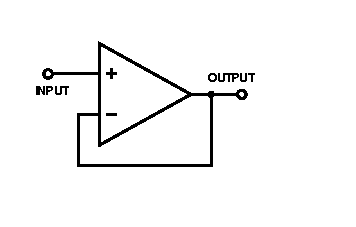
\includegraphics[height=1in]{image/Amp-Follower.pdf}
            \caption{A follower}
            \label{fig:follower}
        \end{figure}{}
        The simplest negative feedback circuit is a follower, so as in Figure~\ref{fig:follower}. From Equation~\ref{eq:veq}, we see that
        \begin{equation}
            V_\text{out} = V_\text{in}
        \end{equation}
    \subsection{Inverting Amplifier}
        \begin{figure}[h]
            \centering
            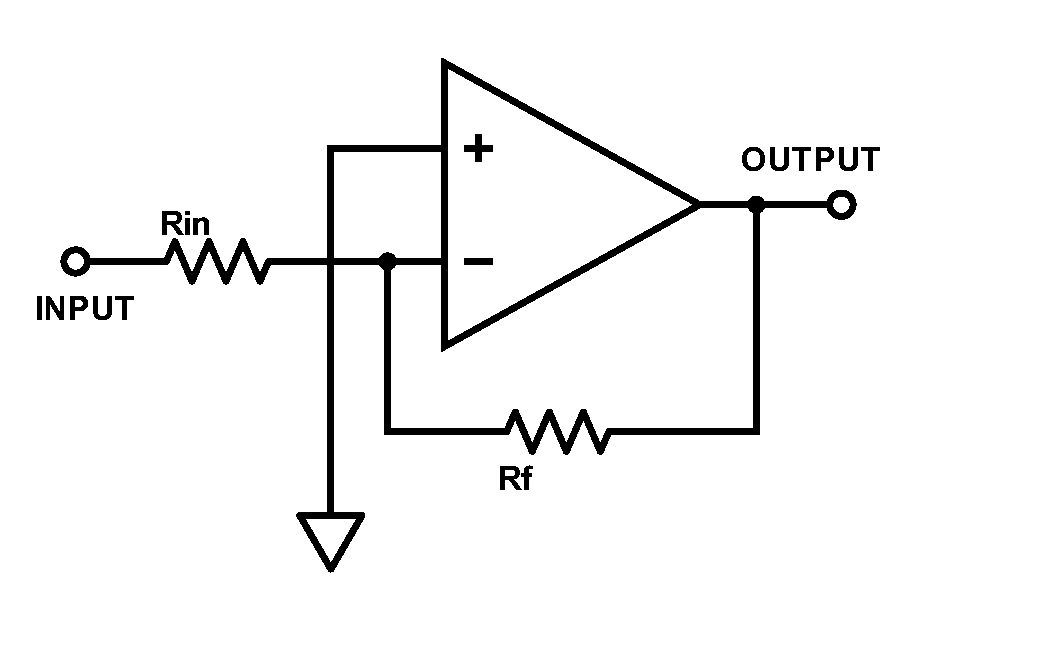
\includegraphics[height=1in]{image/Inverting-Amp.pdf}
            \caption{An Inverting Amplifier}
            \label{fig:invertingAmplifier}
        \end{figure}{}
        An operational amplifier have to be able to be an amplifier! An Inverting Amplifier is presented as Figure~\ref{fig:invertingAmplifier}. Since the non-inverting input is grounded, we must have $v_+ = v_- = 0$V. Thus, we can find the current in the input side are given as
        \[
        I_\text{in} = \frac{V_\text{in}}{R_\text{in}}
        \]
        Follow the Equation~\ref{eq:ieq}, this current have to be also go through $R_f$, where the voltage drop on $R_f$ just so happened to be output voltage ($v_- - V_\text{out}$):
        \begin{align}
            V_\text{out} = - I R_f = - V_\text{in}\frac{R_f}{R_\text{in}} \label{eq:invertingAmplifier}
        \end{align}
        where we see that the gain is just given as:
        \[
            \text{Gain} = - \frac{R_f}{R_\text{in}}
        \]
        Notice that for the inverting amplifier, the input impedance is give as:
        \begin{align*}
            Z_\text{in} = \frac{\de V_\text{in}}{\de I_\text{in}} = R_\text{in}
        \end{align*}
        which is not a very high input impedance. In the other hand, easy to see the output impedance is ideal.

    \subsection{Non-inverting Amplifier}
        \begin{figure}[h]
            \centering
            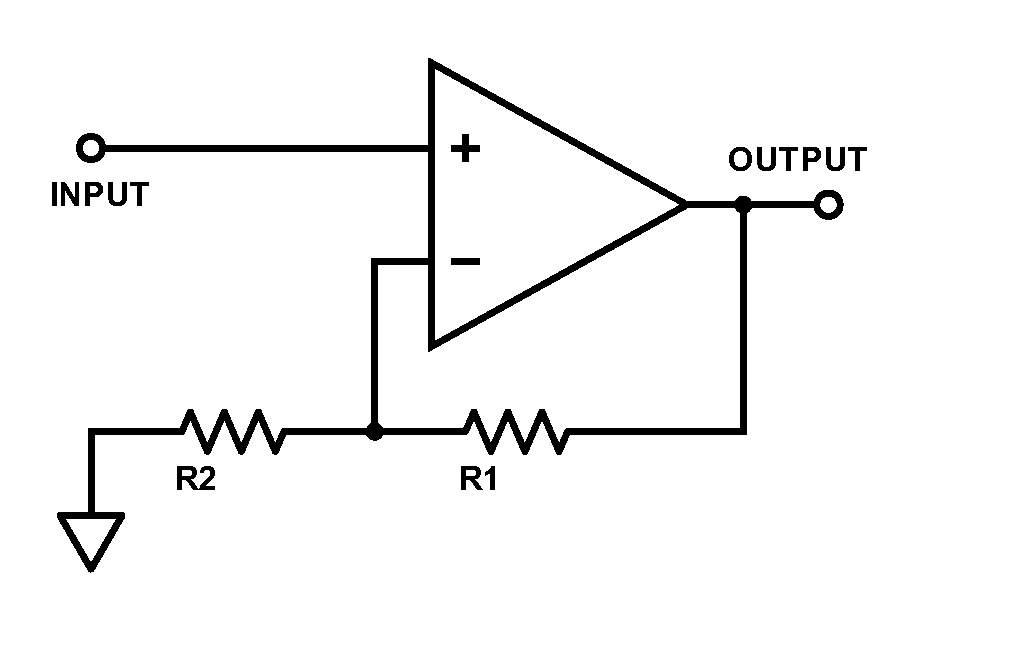
\includegraphics[height=1in]{image/Non-inverting-Amp.pdf}
            \caption{An non-inverting Amplifier}
            \label{fig:nonInvertingAmplifier}
        \end{figure}{}
        It is nice to have a non-inverting amplifier. A non-inverting amplifier is shown as Figure~\ref{fig:nonInvertingAmplifier}. Since the input is directly connect to the non-inverting input, we have $V_\text{input} = v_+ = v_-$. In the end of $R_2$, we must have 0V sicne it is grounded. Thuse we have:
        \[
            I_2 = \frac{V_\text{in}}{R_2}
        \]
        From Equation~\ref{eq:ieq}, this current have to go through $R_1$:
        \[
            V_1 = I R_1 = V_\text{in} \frac{R_1}{R_2}
        \]
        where the other end of $R_2$ just so happened to be the output:
        \begin{equation}
            V_\text{output} = V_\text{in} + V_1 =  V_\text{in} (1+ \frac{R_1}{R_2}) \label{eq:nonInvertingAmplifier}
        \end{equation}
        which give as a gain as:
        \[
            \text{Gain} = (1+ \frac{R_1}{R_2})
        \]

    \subsection{Integrator}
        \begin{figure}[h]
            \centering
            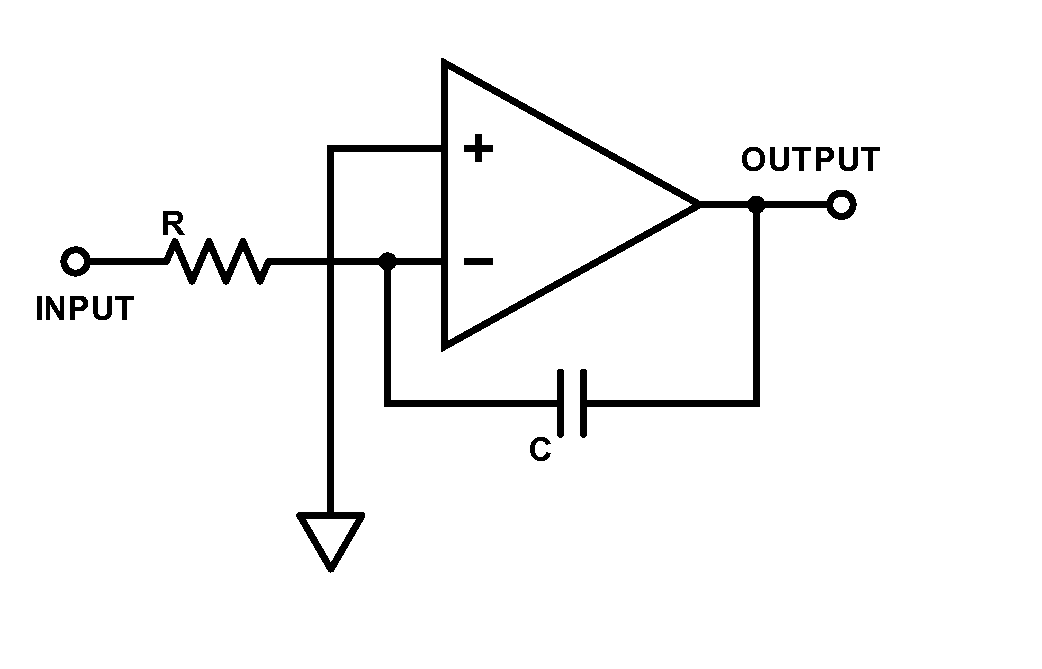
\includegraphics[height=1in]{image/Integrator.pdf}
            \caption{An Integrator}
            \label{fig:integrator}
        \end{figure}{}
        The circuit presented in Figure~\ref{fig:integrator} is an integrator. Since the non-inverting input is grounded, we have $v_- = v_+ = 0$V. Thus we can find the current in the capacitor is the same as the current go through the resistor:
        \[
        I = -C \frac{\de V_\text{out}}{\de t} = \frac{V_\text{in}}{R}
        \]
        solve the equation, we have:
        \begin{equation}
            V_\text{out} = - \frac{1}{RC} \int V_\text{in} \de t \label{eq:integrator}
        \end{equation}

        However, there is a problem for the integrator. Usually, the input might have an offset. That is to say, there is a constent term in the input voltage. This will give us a growing or falling output after integration. To solve it, one can parallel a resistor with the capacitor.
        \subsubsection{T Network}
            \begin{figure}[h]
                \centering
                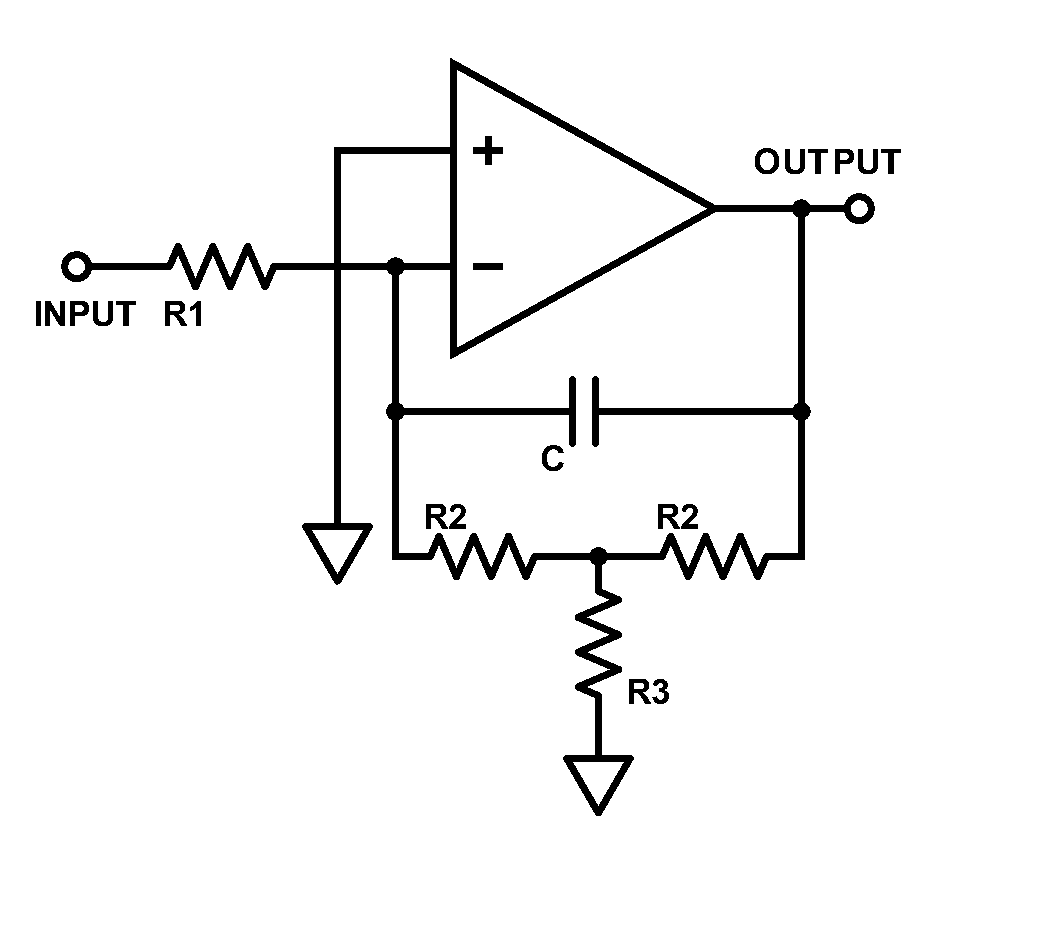
\includegraphics[height=1.3in]{image/T-network.pdf}
                \caption{An Integrator with T network}
                \label{fig:tNetwork}
            \end{figure}{}
            To achieve a large parallel resistor, one can use a T network, so as in Figure~\ref{fig:tNetwork}. Ignore the capacitor, we can just calculate the effect of the T network. First, we still have the current on the $R_1$ will go through the left $R_2$:
            \[
            I_1 = \frac{V_\text{in}}{R_1} = I_\text{2L} = I_\text{2R} + I_3
            \]
            On the other hand, the voltage between $R_1$ and $R_\text{2L}$ is 0V. Thus we can find the voltage between two $R_2$:
            \[
            V_2 = 0 - I_1 R_2 = - V_\text{in} \frac{R_2}{R_1}
            \]
            And this voltage will dorp to zero once it go through $R_3$:
            \[
            I_3 = \frac{V_2}{R_3} = - V_\text{in} \frac{R_2}{R_1 R_3}
            \]
            In the output end, we can write the current go through $R_2$ as following:
            \[
            I_2 = \frac{V_2 - V_\text{out}}{R_2} = -\frac{V_\text{in}}{R_1} - \frac{V_\text{out}}{R_2}
            \]
            This relate the output voltage to the current. Now we have $I_1 = I_2 + I_3$:
            \[
            \frac{V_\text{in}}{R_1} =  - V_\text{in} \frac{R_2}{R_1 R_3} -\frac{V_\text{in}}{R_1} - \frac{V_\text{out}}{R_2}
            \]
            Solve the equation, we find
            \[
            V_\text{out} = - V_\text{in} \frac{R_2}{R_1} (2 + \frac{R_2}{R_3})
            \]
            This give us the impedance of the T network:
            \[
            Z_f = R_2(2 + \frac{R_2}{R_3})
            \]
            Thus, we can achieve a high impedance if we just chose two two small resistor with a large ratio.
    \subsection{Differentiator}
        \begin{figure}[h]
            \centering
            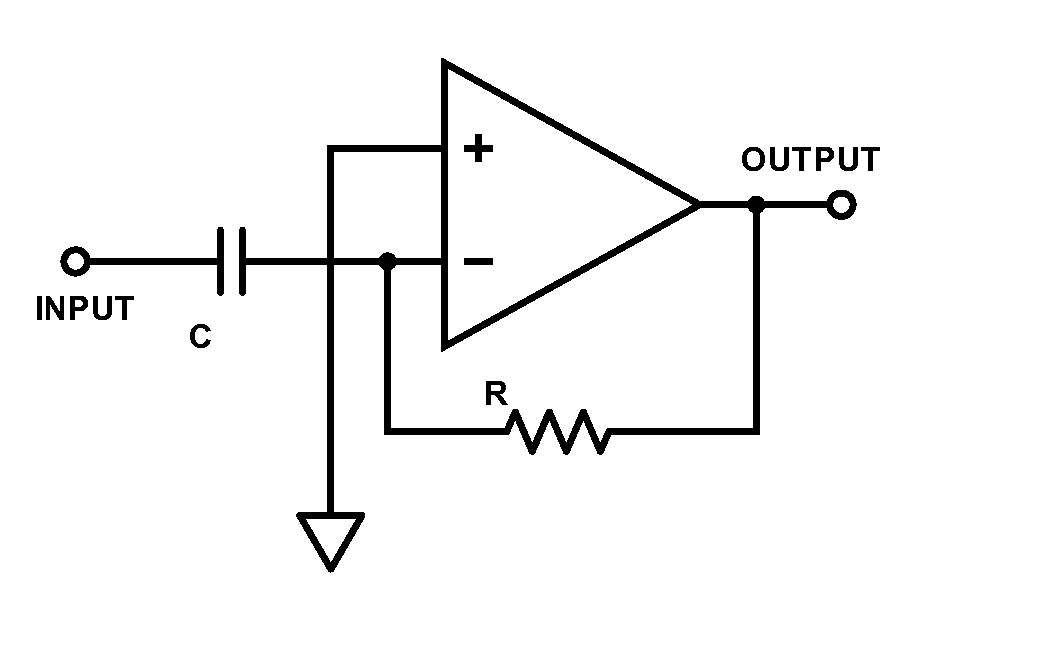
\includegraphics[height=1in]{image/Differentiator.pdf}
            \caption{An Differentiator}
            \label{fig:differentiator}
        \end{figure}{}
        By interchange the resistor and capacitor of integrator, one can achieve a differentiator, as in Figure~\ref{fig:differentiator}. Since the non-inverting input is grounded, we have to have 0V on $v_-$. This means the current go through the capacitor and the resistor are the same:
        \begin{equation}
            V_\text{out} = - IR = -RC \frac{\de V\text{in}}{\de t}
        \end{equation}

    \subsection{Limit of the Opamp}
        A realistic opamp are not ideal. There are a few importent things we have to consider when use it:
        \begin{enumerate}
            \item The voltage gain ($A_0$) will drop linearly to the frequency in logarithm scale;
            \item There might be a phase shift in the output;
            \item For the feedback loop, Equation~\ref{eq:ieq} is approximate, i.e., $i_+$, $i_- \approx 0$;
            \item For the feedback loop, Equation~\ref{eq:veq} is approximate, i.e., $v_+ \approx v_-$;
            \item There is a small delay to the output. When input voltage change suddenly, the output voltage will learly increase and reach the theoretical value. This is called slew rate.
        \end{enumerate}
\section{Data and Calculation}
    \subsection{Follower}
        \begin{figure}[h]
            \centering
            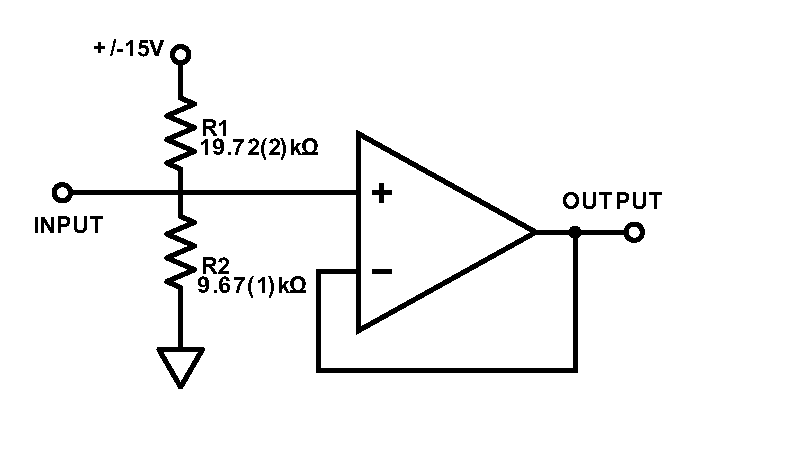
\includegraphics[height=1in]{image/follower/Amp-Follower-Lab.pdf}
            \caption{An follower with changeable DC input}
            \label{fig:followerLab}
        \end{figure}{}

        \begin{figure}[t]
            \centering
            \subcaptionbox{1kHz}[.49\linewidth][c]{%
                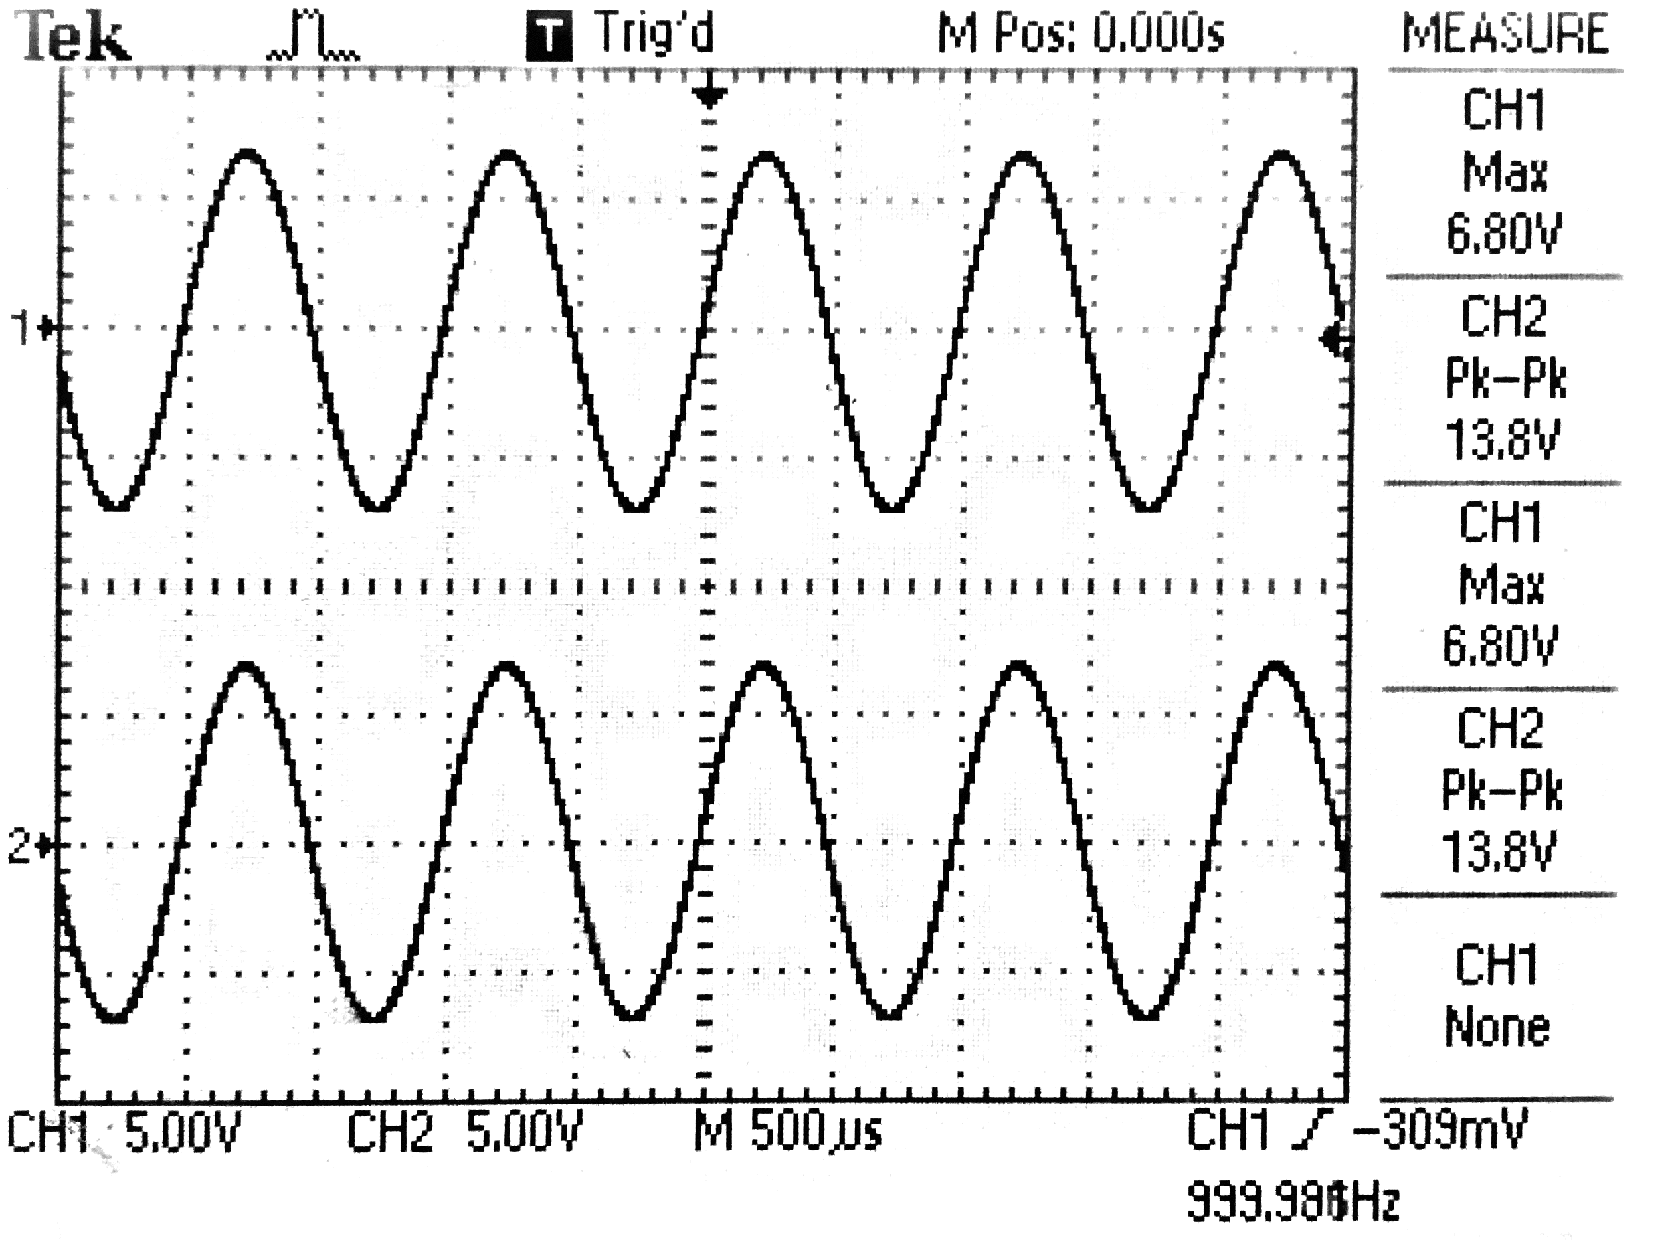
\includegraphics[width=.49\linewidth]{image/follower/1kHz.pdf}}\ 
            \subcaptionbox{100kHz}[.49\linewidth][c]{%
                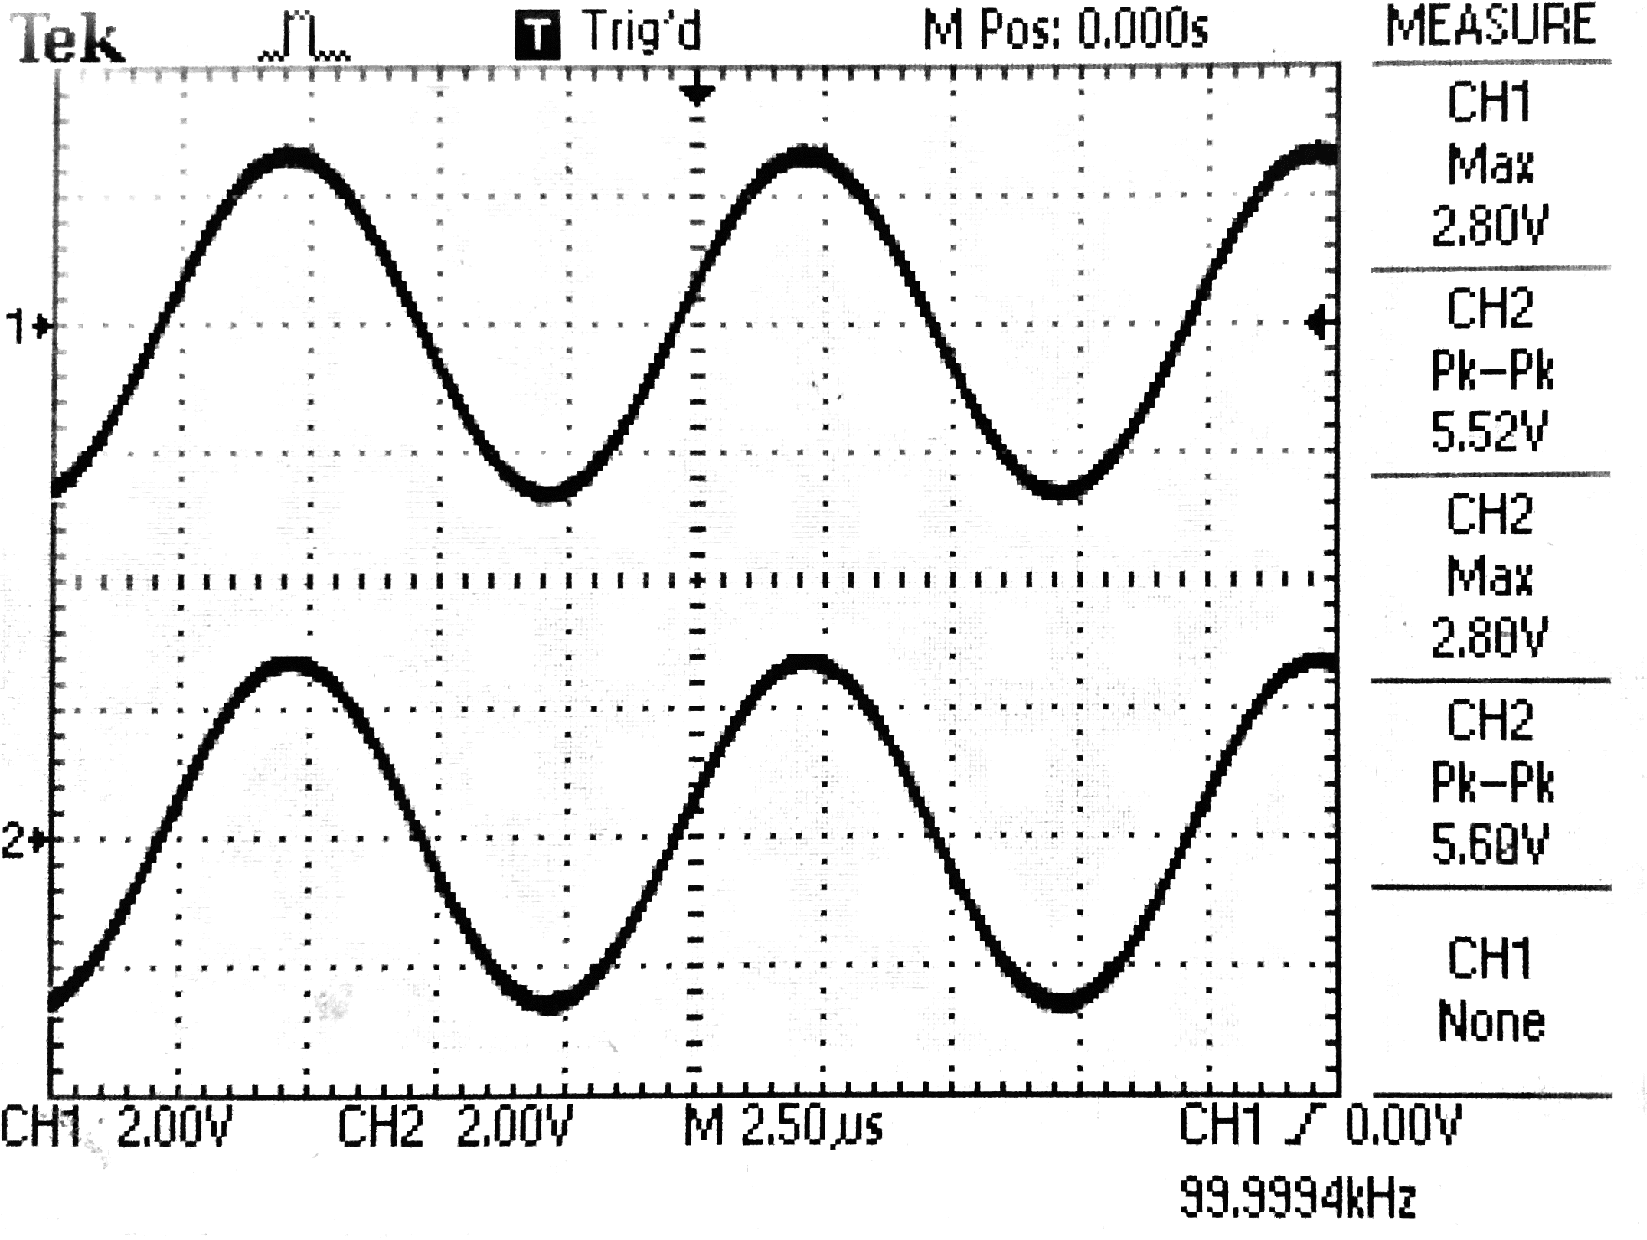
\includegraphics[width=.49\linewidth]{image/follower/100kHz.pdf}}\ 
            \caption{The input and the ouput voltage for the follower in different frequency}
        \end{figure}
        In this part we build a follower as in Figure~\ref{fig:followerLab}. The resistor is actualy changeable so that we can achieve different voltage. By let the ratio of two resistor is up to 1:2, we can change our input DC voltage from -5V to 5V. The data obtained is in appendix, where the frequency is record as "DC". We can also remove the voltage divider and directly use a input from signal generator so as in Figure~\ref{fig:follower}, the data obtained also presented in the appendix.

        On the other hand, to see that the impedance of the circuit is ideal, we can link a 1.12(1)k$\Omega$ load resistor in the output end of the Figure~\ref{fig:followerLab}. The value of the resistor for this part is shown in the Figure~\ref{fig:followerLab}: $R_1 = 9.67(1)$k$\Omega$, and $R_2 = 19.72$k$\Omega$. When we use this circuit, wee find the input voltage is 15.2(2)V with a 10.6(2)V output. However, when we remove the follower, we have a 1.42(2)V output.
    \subsection{Amplifier}
        \begin{figure}[h]
            \centering
            \subcaptionbox{Non-inverting}[.45\linewidth][c]{%
                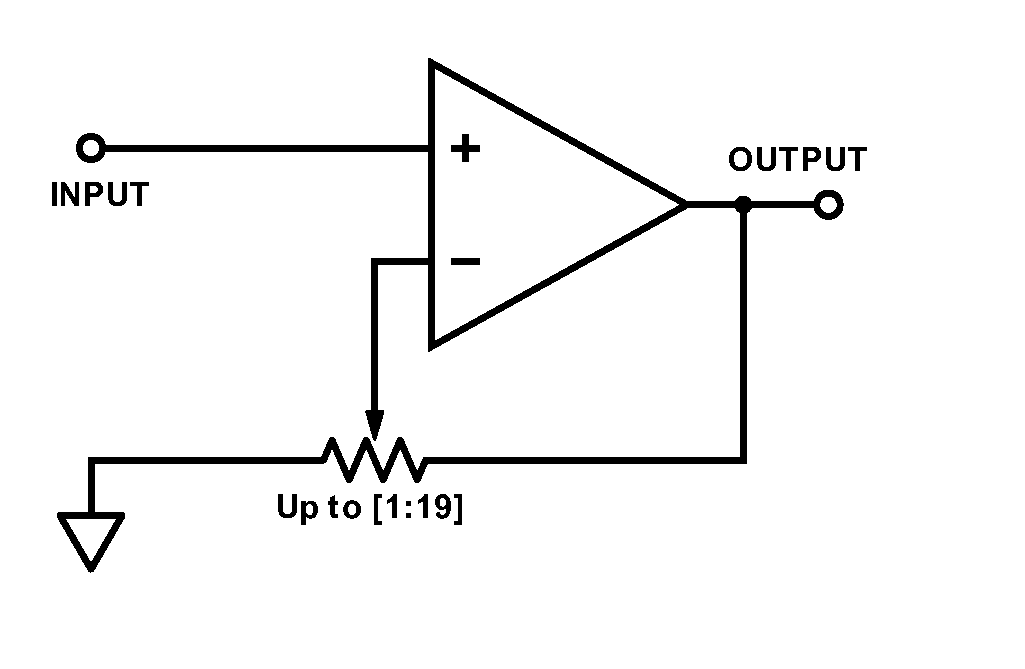
\includegraphics[width=.4\linewidth]{image/amp/Non-inverting-Amp-Lab.pdf}}\ 
            \subcaptionbox{Inverting}[.45\linewidth][c]{%
                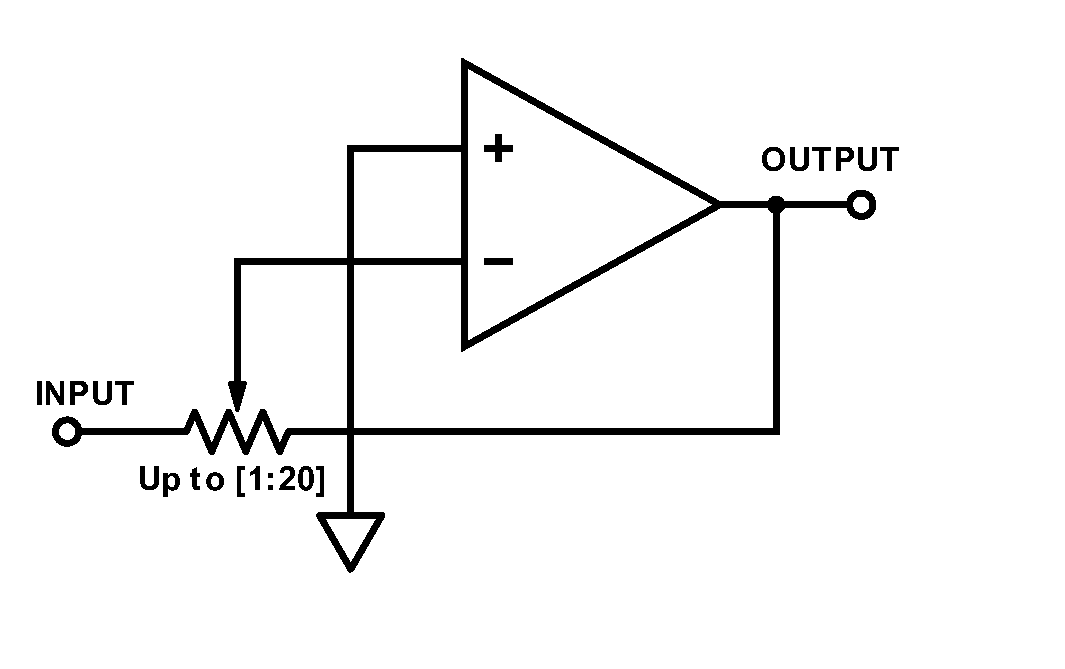
\includegraphics[width=.4\linewidth]{image/amp/Inverting-Amp-Lab.pdf}}
            \subcaptionbox{The output of inverting Amplifier at 1kHz}[\linewidth][c]{%
                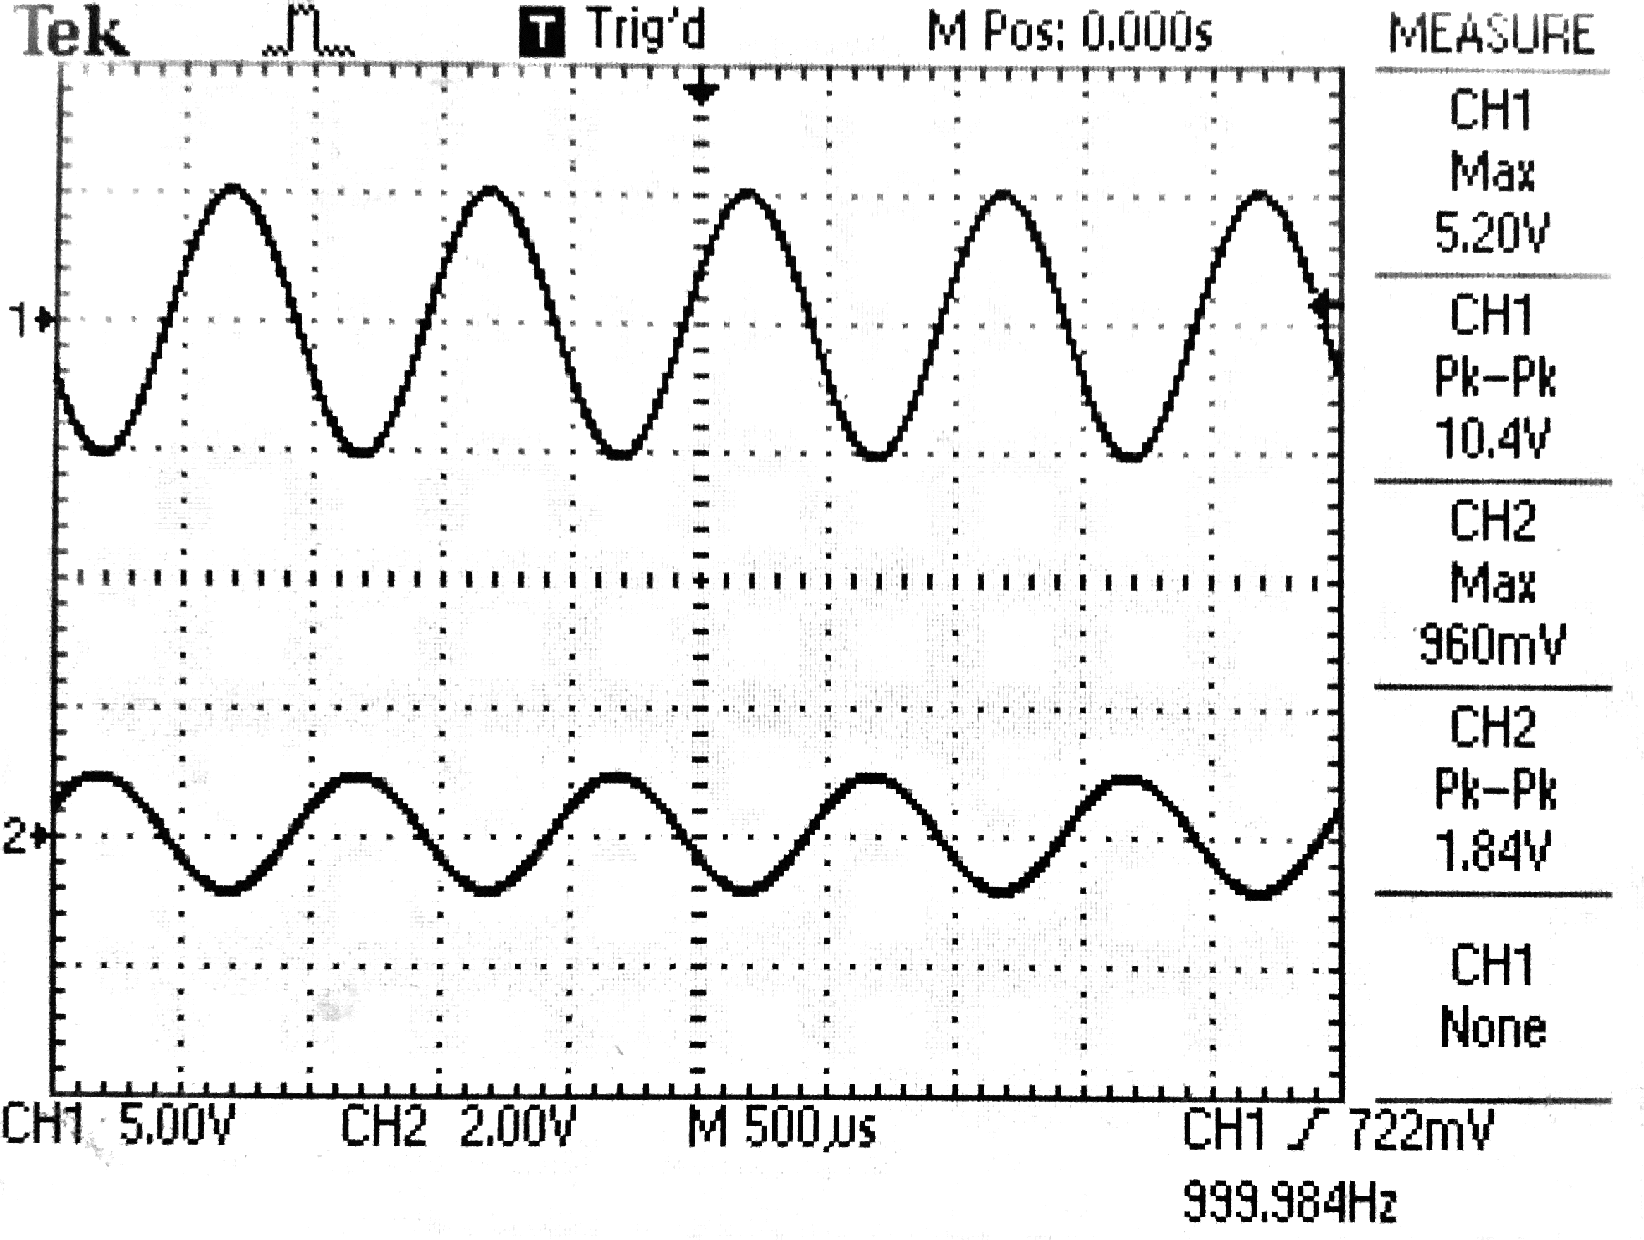
\includegraphics[width=0.7\linewidth]{image/amp/inv.pdf}}
            \caption{The amplifier circuit used in lab and its output}
            \label{fig:amplifierLab}
        \end{figure}
        In the lab we use a 10k$\Omega$ potentiometer to achieve the amplifier with different gain. In here we want to achieve the highest gain is 26dB, i.e., the gain is around 20. Following the Equation~\ref{eq:invertingAmplifier} and Equation~\ref{eq:nonInvertingAmplifier}, we want the ratio of the resistor is up to 1:19 for the non-inverting amplifier and is up to 1:20 for the inverting amplifier. THe circuit used in the lab is presented in the Figure~\ref{fig:amplifierLab}.

        In the lab, we measure the 3 different set of data for different gain for each amplifier. The data obtained is in the appendix.
    \subsection{Integrator}
        \begin{figure}[h]
            \centering
            \subcaptionbox{Without T network}[.45\linewidth][c]{%
                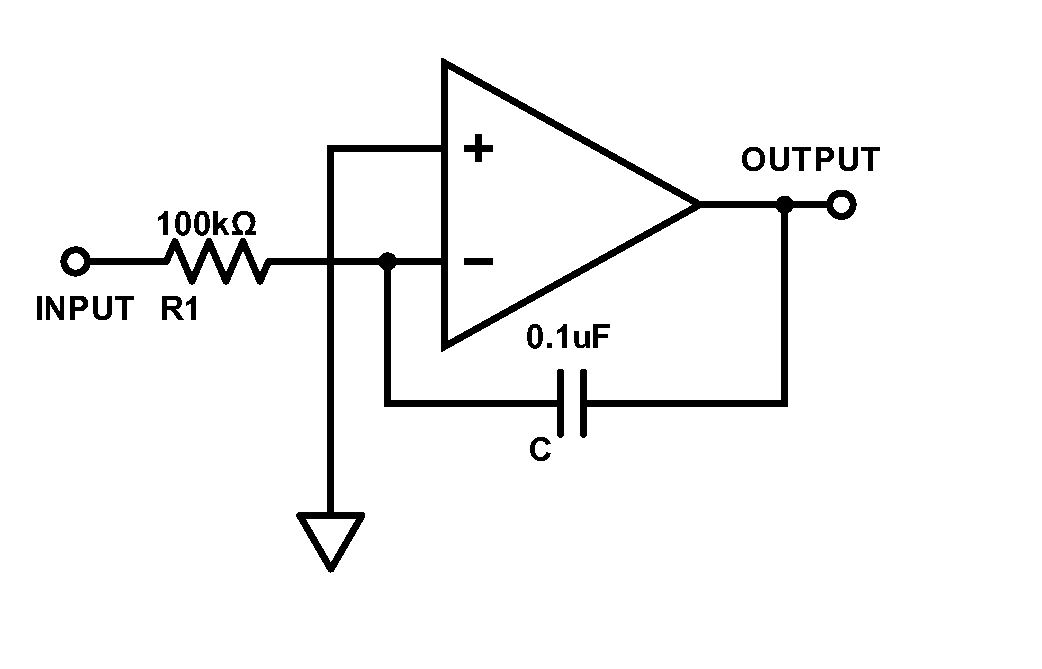
\includegraphics[width=.4\linewidth]{image/integrator/Integrator-Lab.pdf}}\ 
            \subcaptionbox{With T network}[.45\linewidth][c]{%
                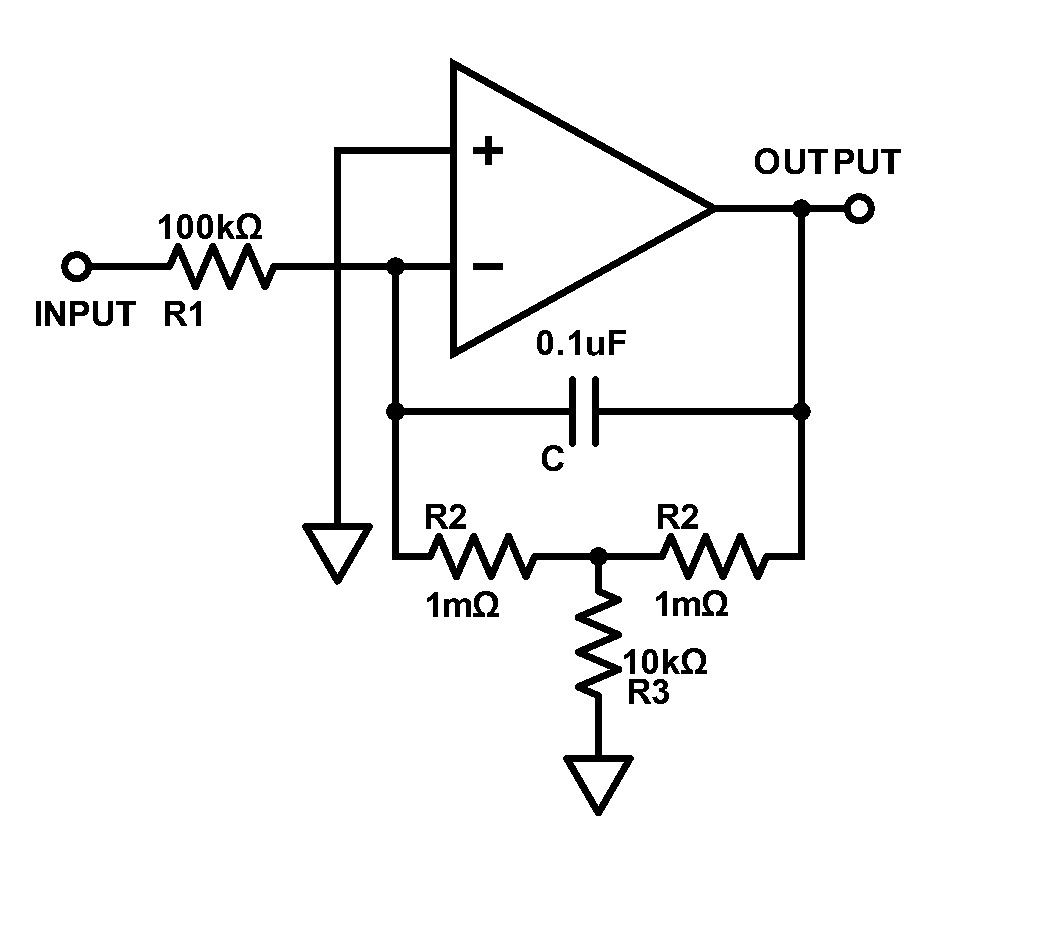
\includegraphics[width=.4\linewidth]{image/integrator/T-network.pdf}}\ 
            \caption{Integrator used in lab}
            \label{fig:integratorLab}
        \end{figure}

        \begin{figure}[b]
            \centering
            \subcaptionbox{Sine wave}[.49\linewidth][c]{%
                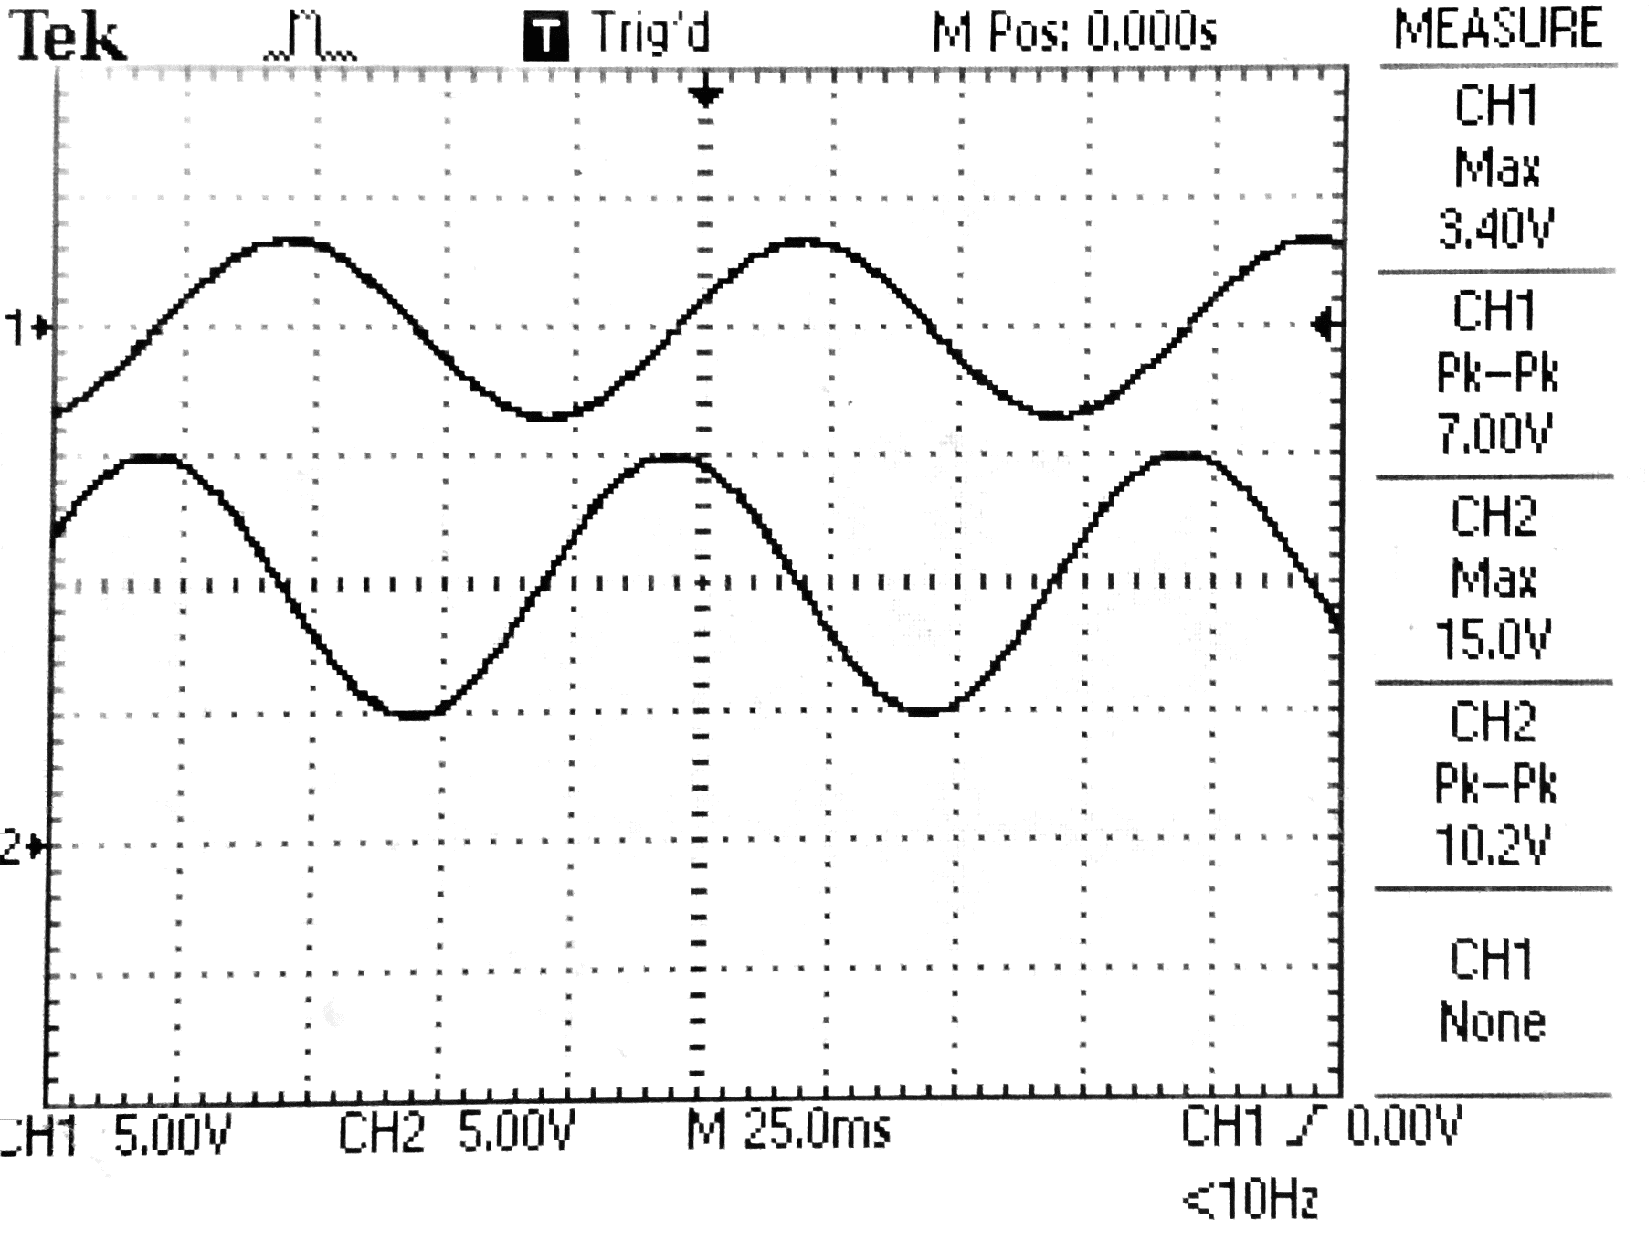
\includegraphics[width=.49\linewidth]{image/integrator/sine.pdf}}
            \subcaptionbox{Triangle wave}[.49\linewidth][c]{%
                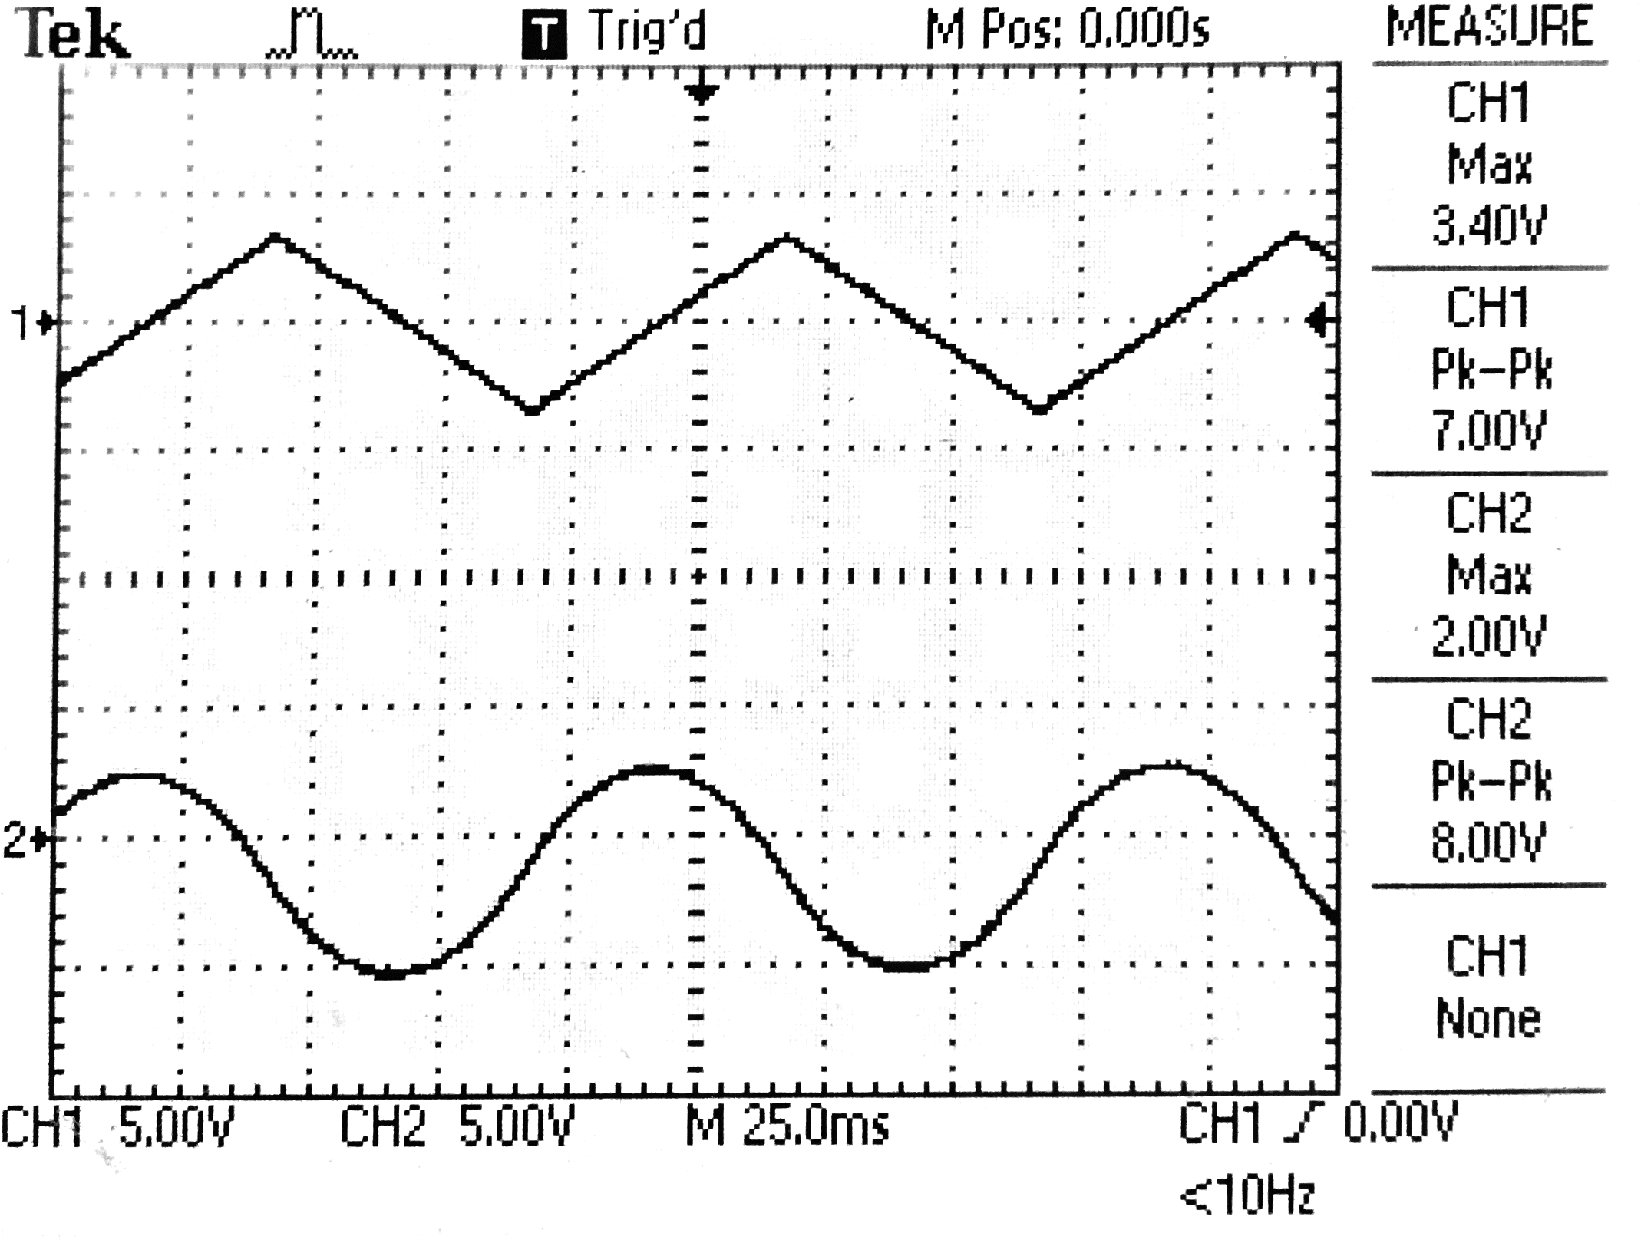
\includegraphics[width=.49\linewidth]{image/integrator/tri.pdf}}
            \subcaptionbox{Square wave}[.49\linewidth][c]{%
                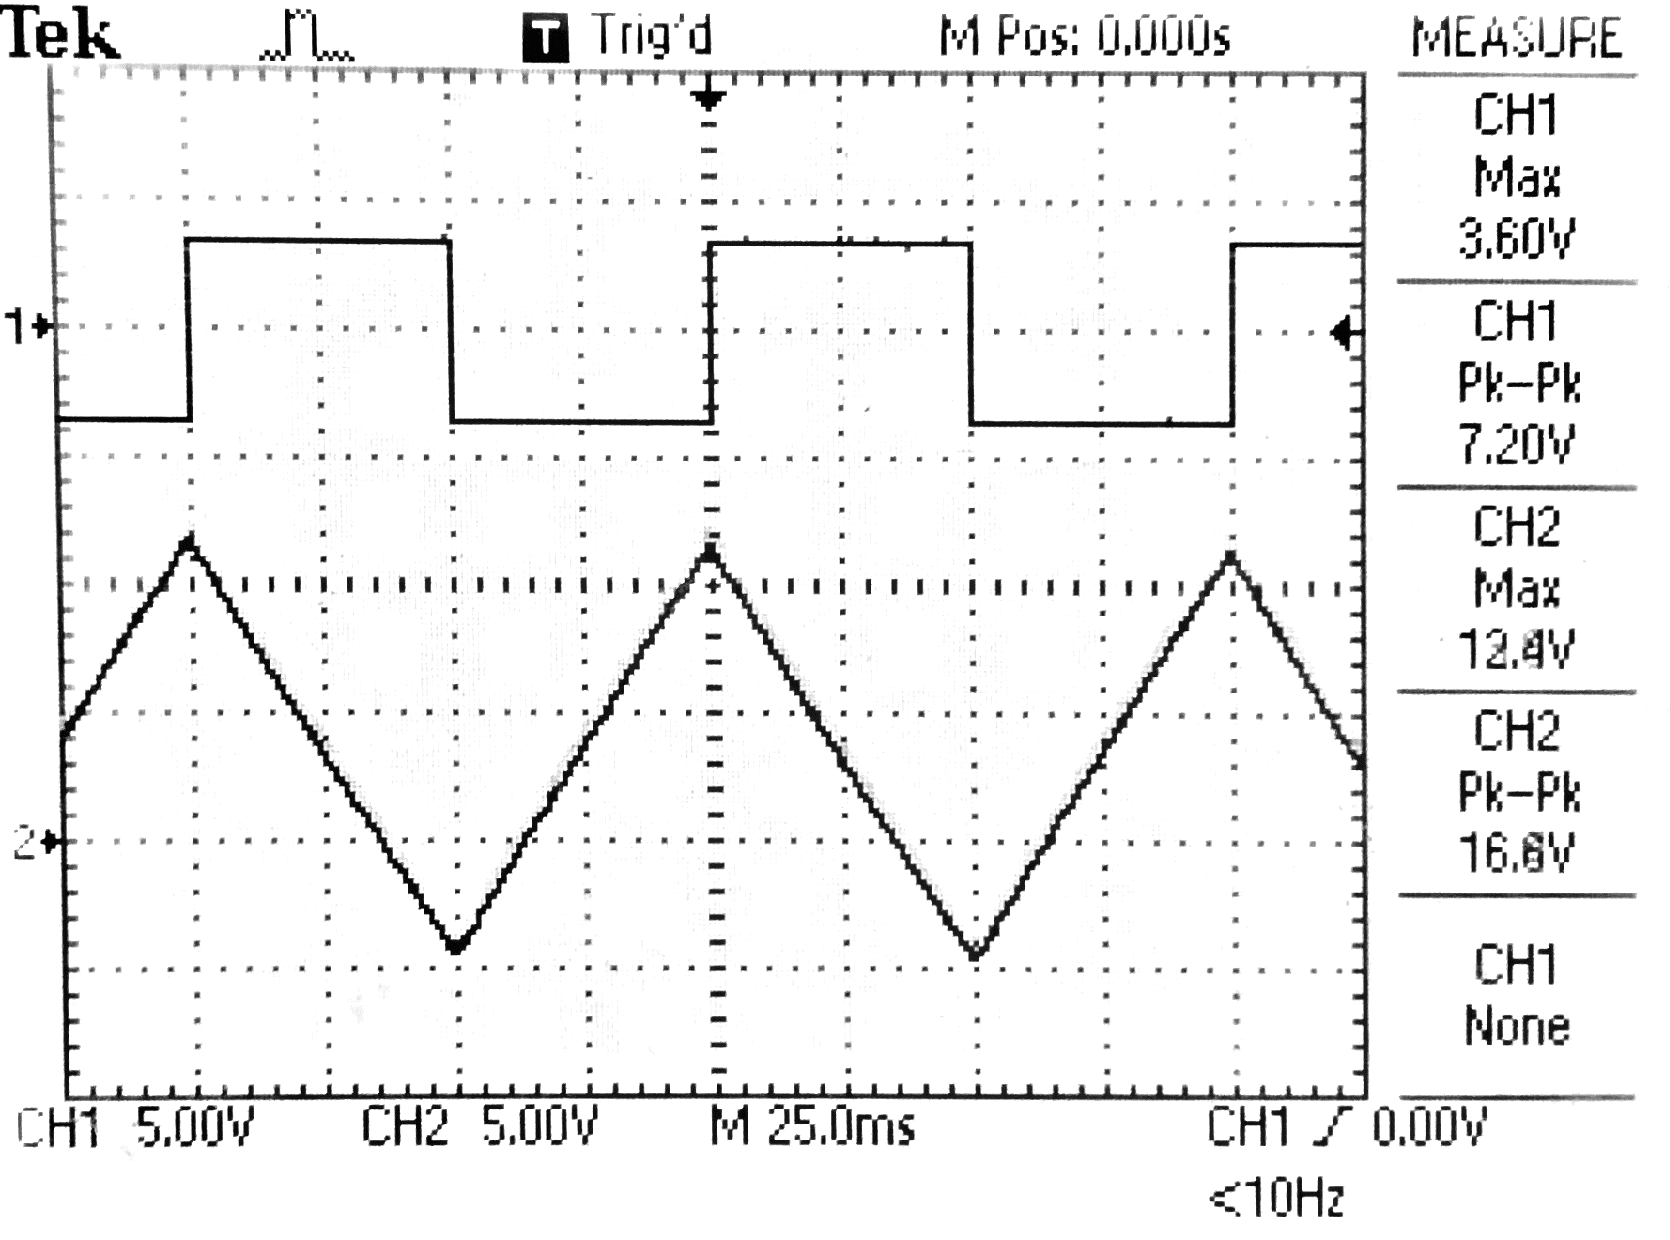
\includegraphics[width=.49\linewidth]{image/integrator/sqr.pdf}}
            \subcaptionbox{Square wave on high frequency}[.49\linewidth][c]{%
                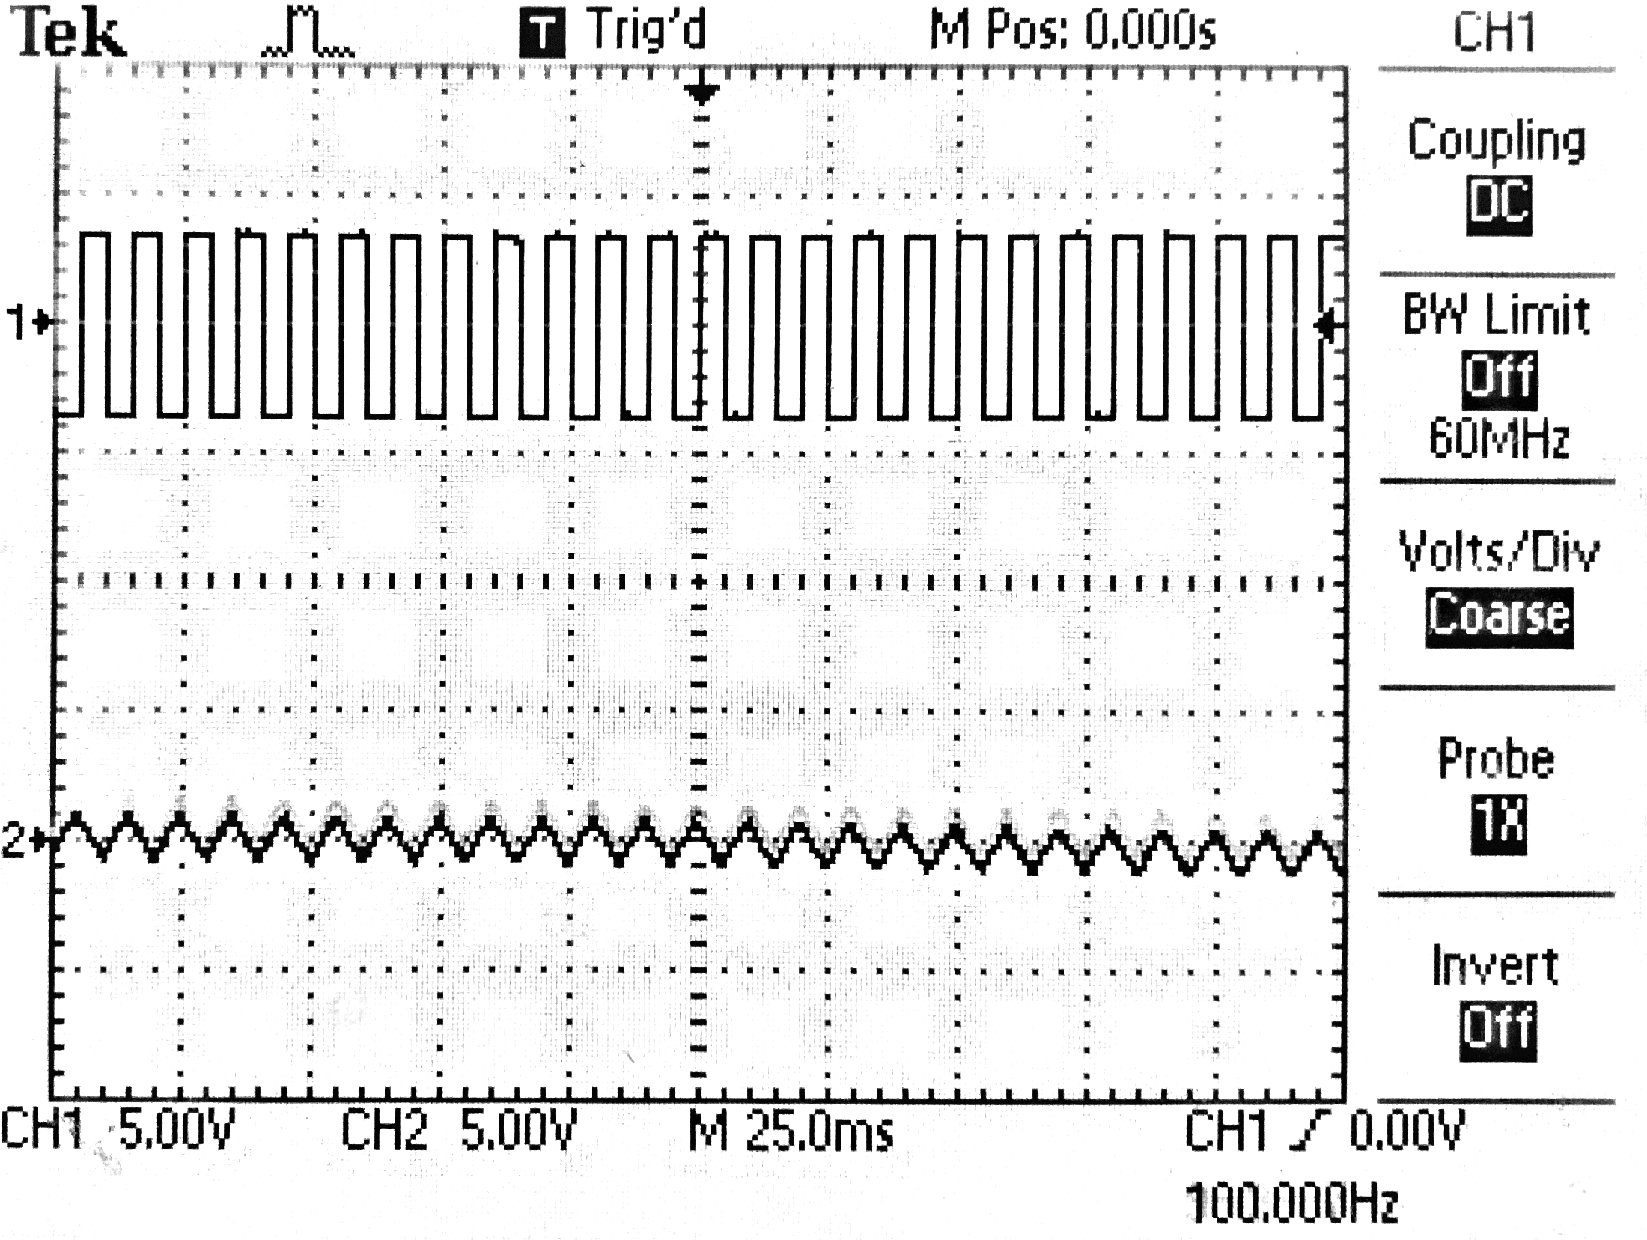
\includegraphics[width=.49\linewidth]{image/integrator/highFre.pdf}}
            \caption{Result of different wave form for integrator}
            \label{fig:integratorWave}
        \end{figure}
        We have used two integrator shown in Figure~\ref{fig:integratorLab}. One is with T network and the other one does not use T network. We chose a 0.1$\mu$F capacitor and a 100k$\Omega$ resistor for the both case.

        For the one without T network, when we connect the input to the ground, we see a upgoing line. On the other hand, we can connect the signal generator to the input. The output voltage shift up and down for different wave form. When frequency increase, the output peak to peak voltage drop significantly. We observed that the output voltage droped below 1V at 100Hz and unrecognizable for the higher frequency.

        For the one with T network, we observed the same shift but the shift is slower. When frequency increase, the output drop below to 1V at 300Hz, and unrecognizable for the higher frequency.

        We also measure the input and the output voltage when input is 1V (2V peak to peak) square wave with different frequency. The output volrage after 500Hz is almost zero and unrecognizable. The data obtained is in appendix.

        For both case, when input voltage have a large amplitude, the output usually be cut off on the $\pm$15V.
    \subsection{Differentiator}
        \begin{figure}[h]
            \centering
            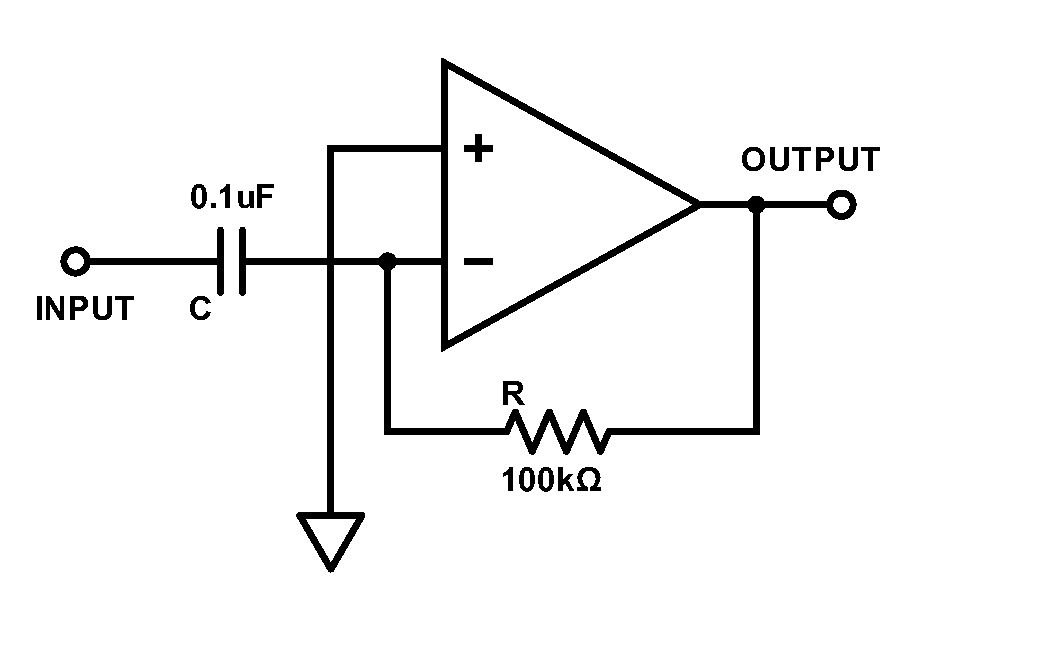
\includegraphics[height=1in]{image/differentiator/Differentiator-Lab.pdf}
            \caption{Differentiator used in lab}
            \label{fig:differentiatorLab}
        \end{figure}{}

        \begin{figure}[b]
            \centering
            \subcaptionbox{Sine wave}[.49\linewidth][c]{%
                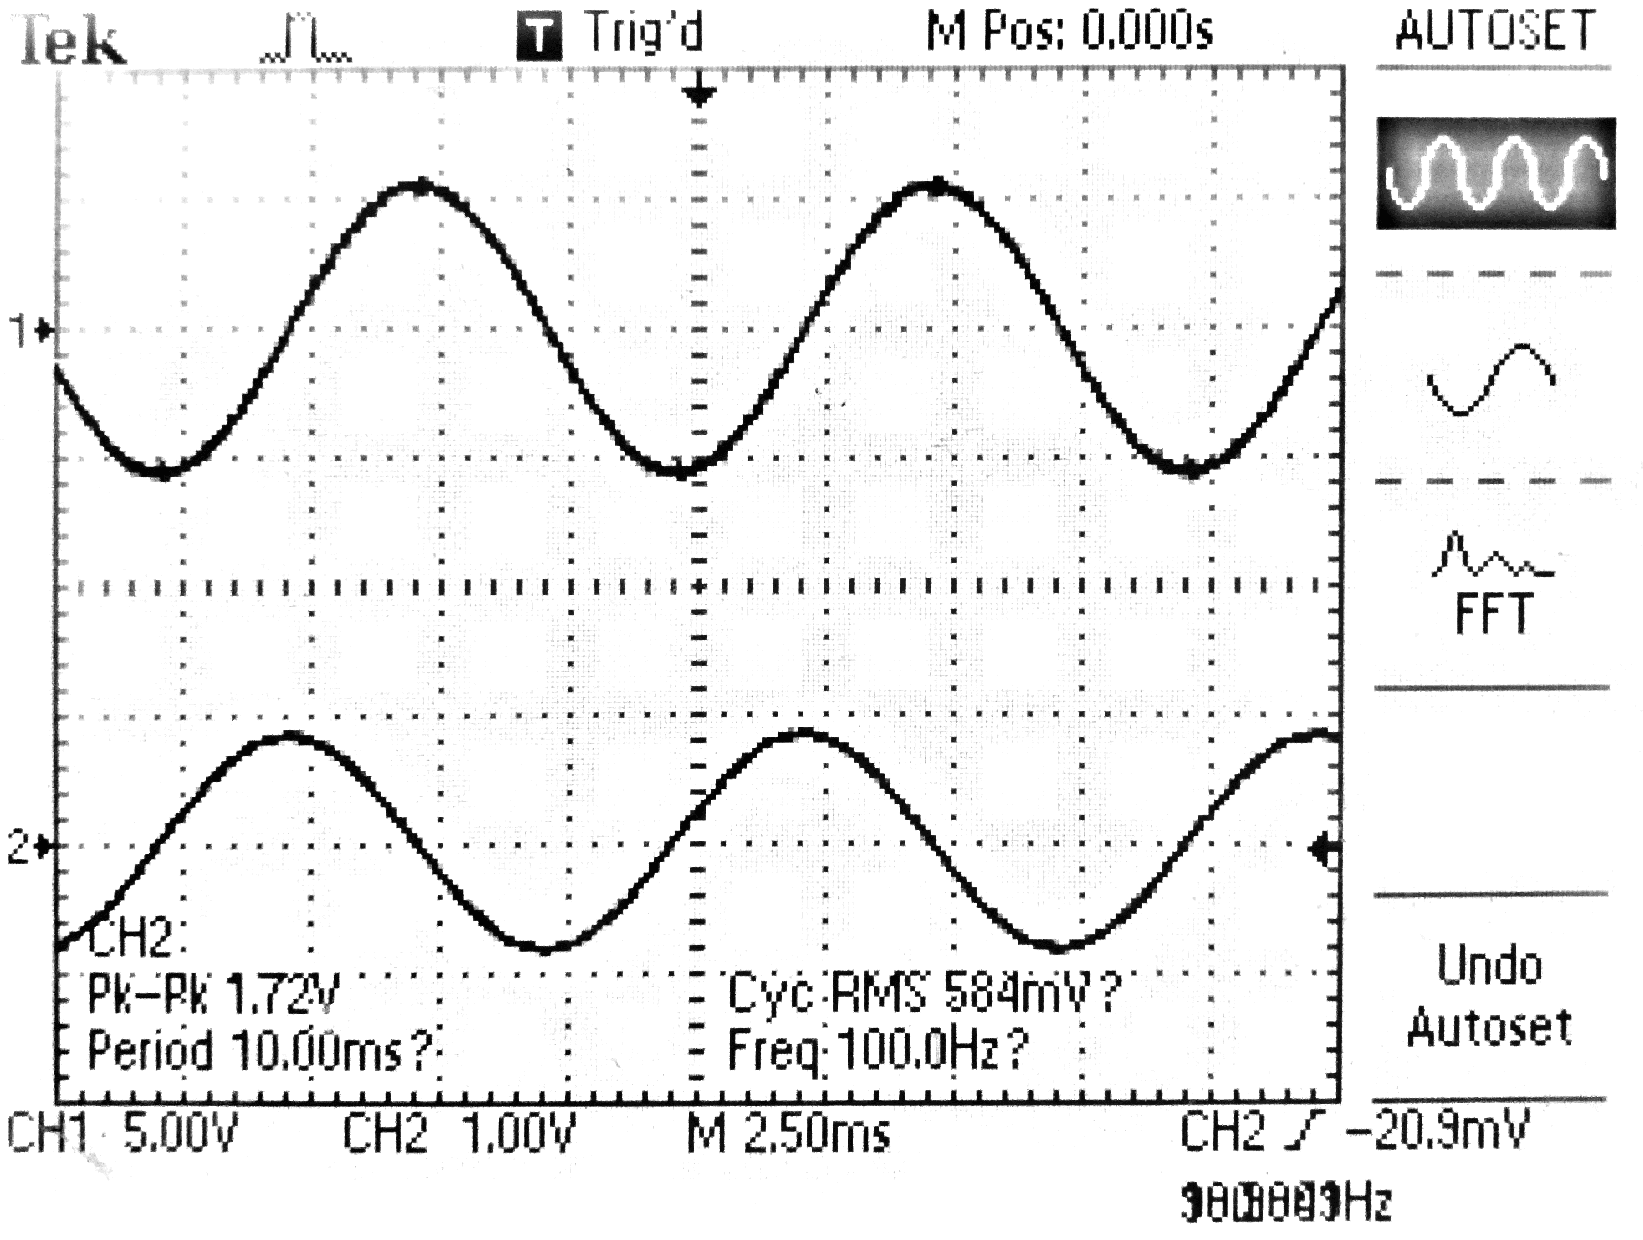
\includegraphics[width=.49\linewidth]{image/differentiator/sine.pdf}}
            \subcaptionbox{Triangle wave}[.49\linewidth][c]{%
                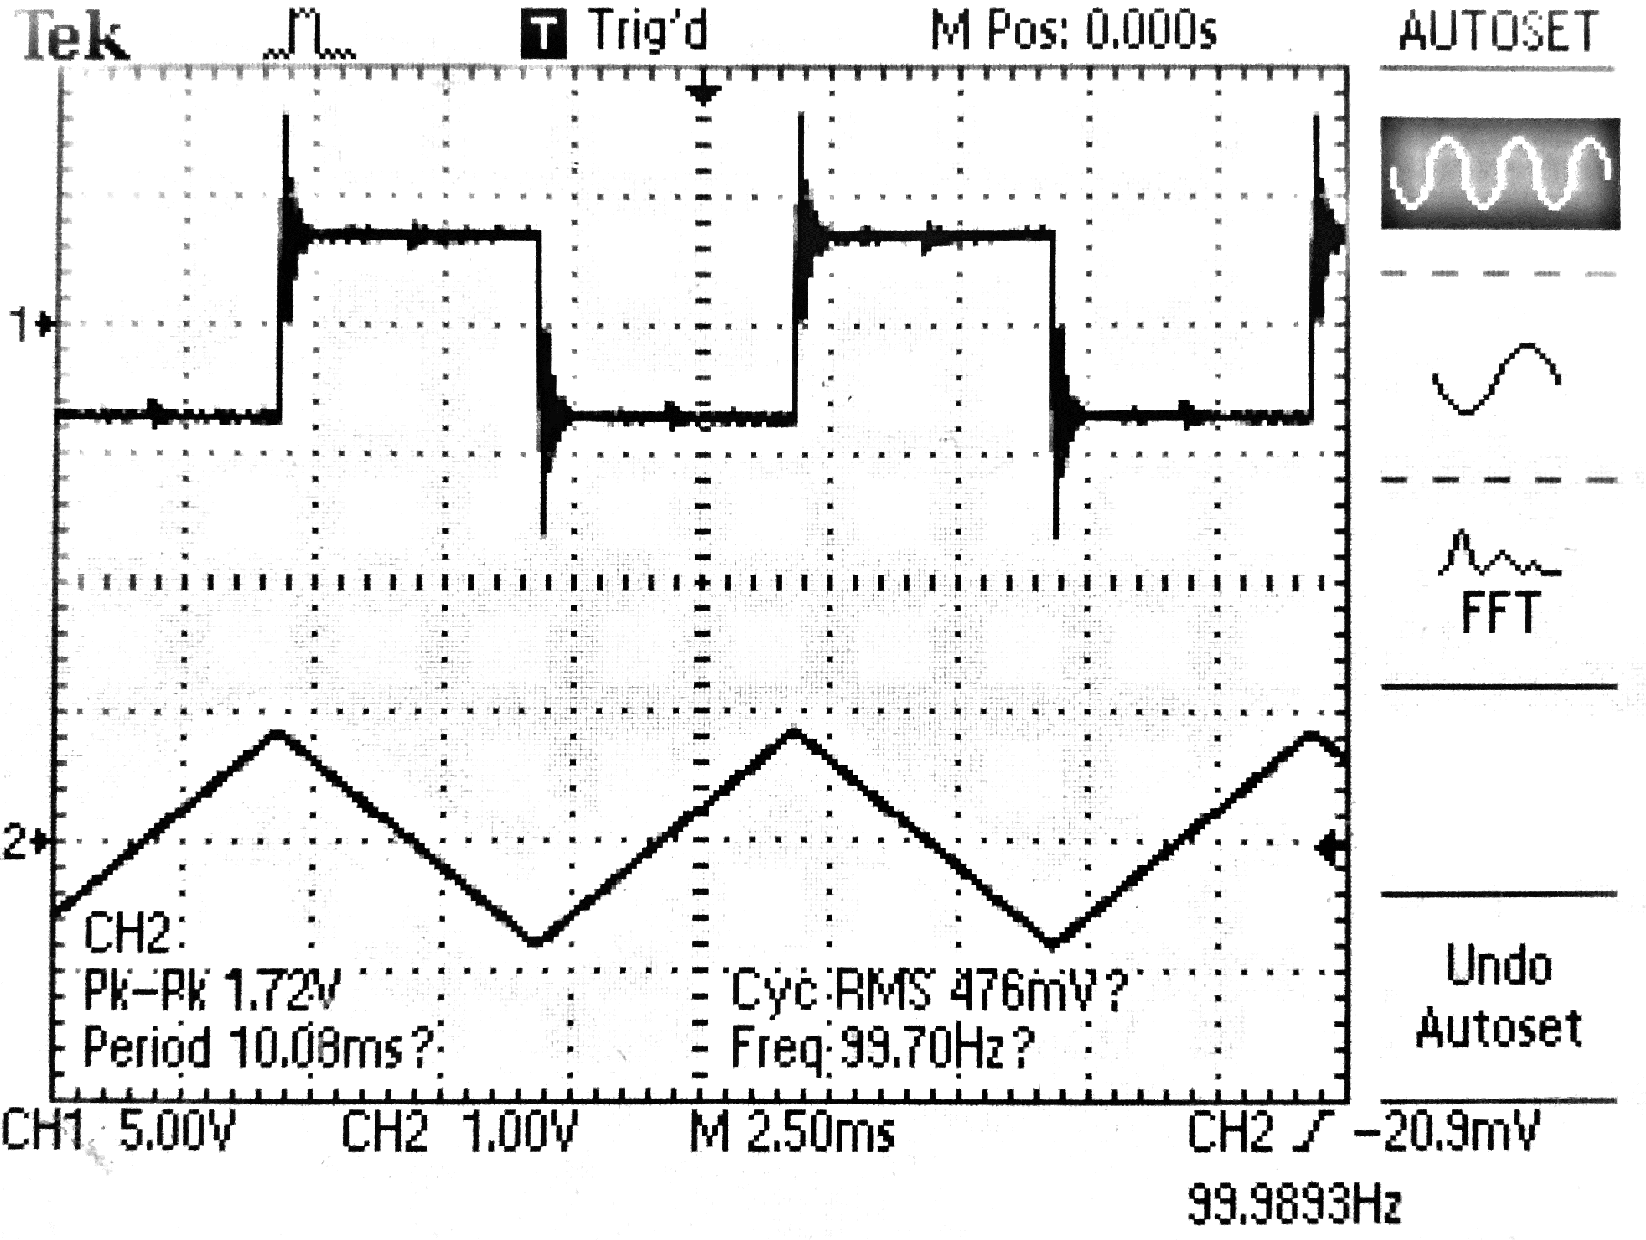
\includegraphics[width=.49\linewidth]{image/differentiator/tri.pdf}}
            \subcaptionbox{Square wave}[\linewidth][c]{%
                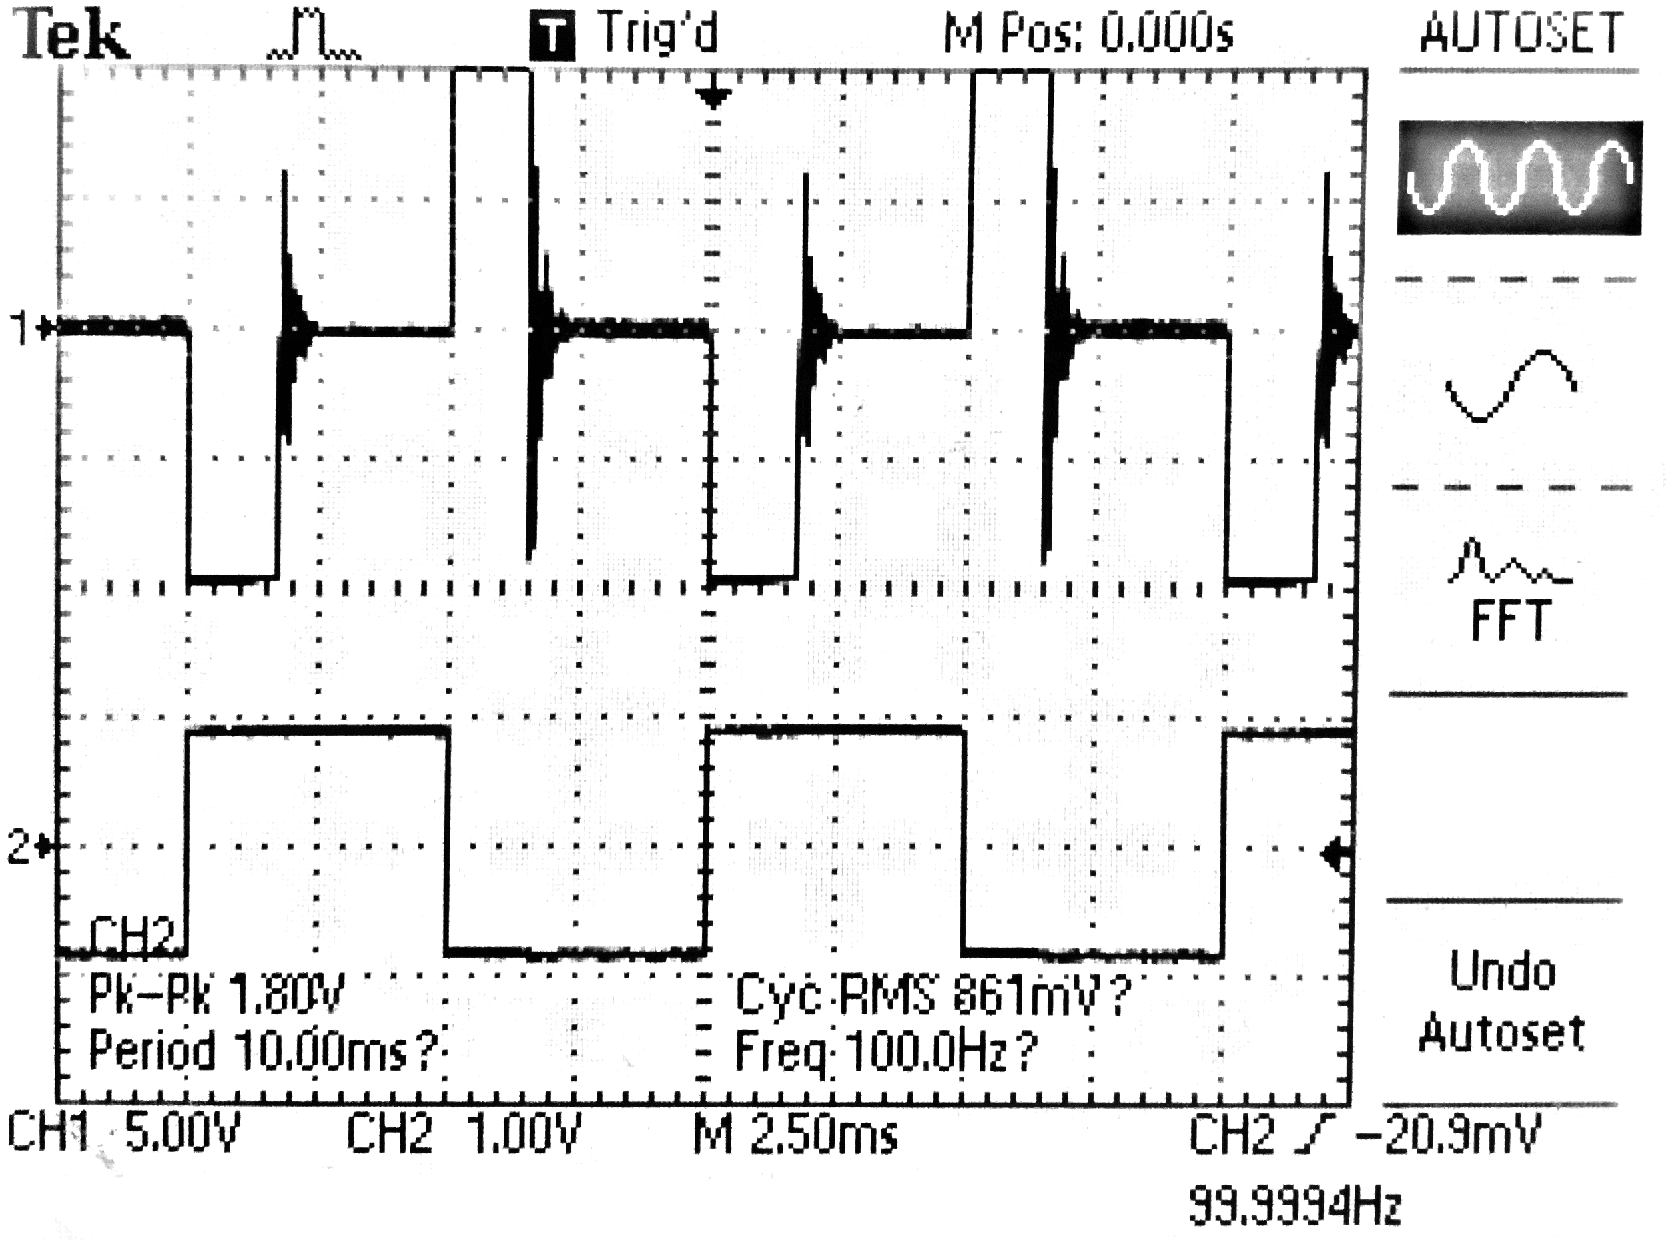
\includegraphics[width=.7\linewidth]{image/differentiator/sqr.pdf}}
            \caption{Result of different wave form for differentiator}
            \label{fig:differentiatorWave}
        \end{figure}
        In the lab we use a Differentiator as in Figure~\ref{fig:differentiatorLab}. We chose a 0.1$\mu$F capacitor and a 100k$\Omega$ resistor. We use a 5V amplitude on the input for all the wave fomr.

    \subsection{Slew Rate}
        To measure the slew rate, there are two different way.
        \begin{figure}[h]
            \centering
            \subcaptionbox{Disform of sine wave}[.49\linewidth][c]{%
                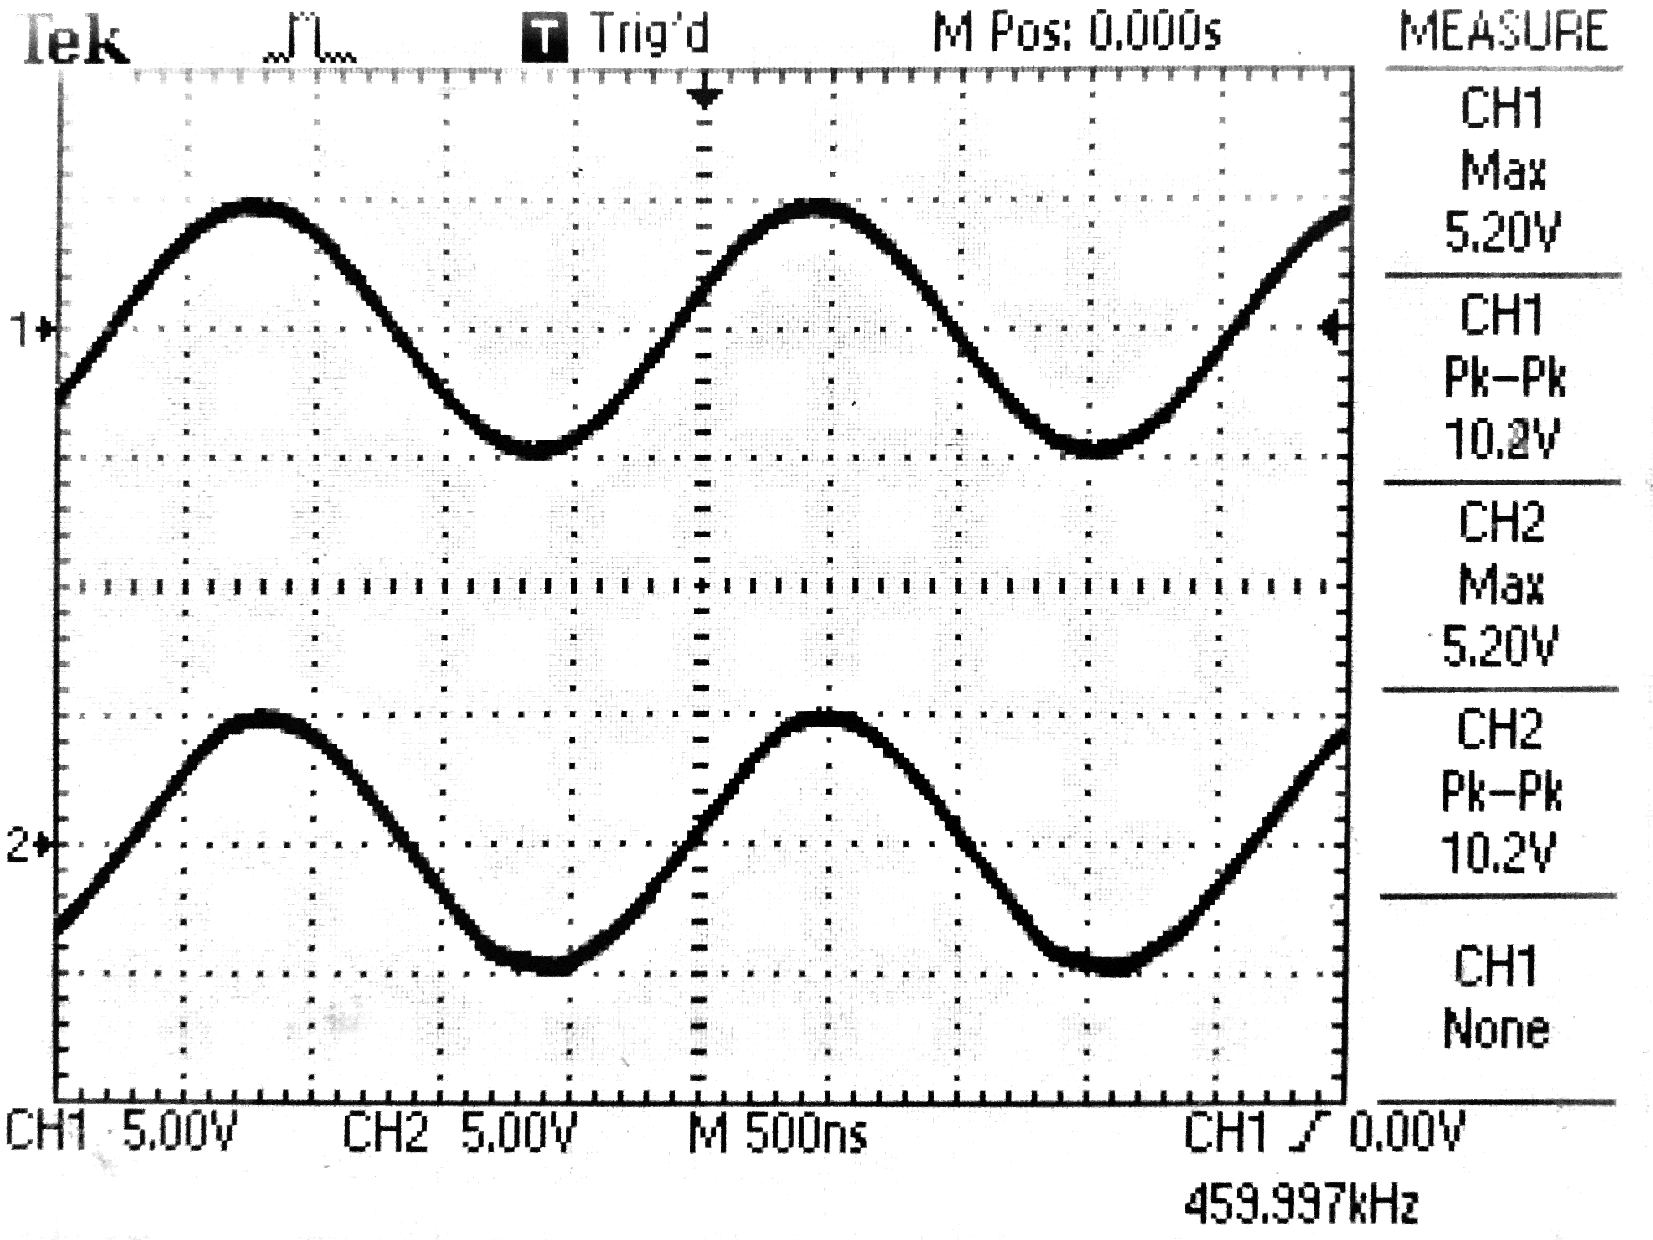
\includegraphics[width=.49\linewidth]{image/rate/wave.pdf}}
            \subcaptionbox{Sudden voltage change}[.49\linewidth][c]{%
                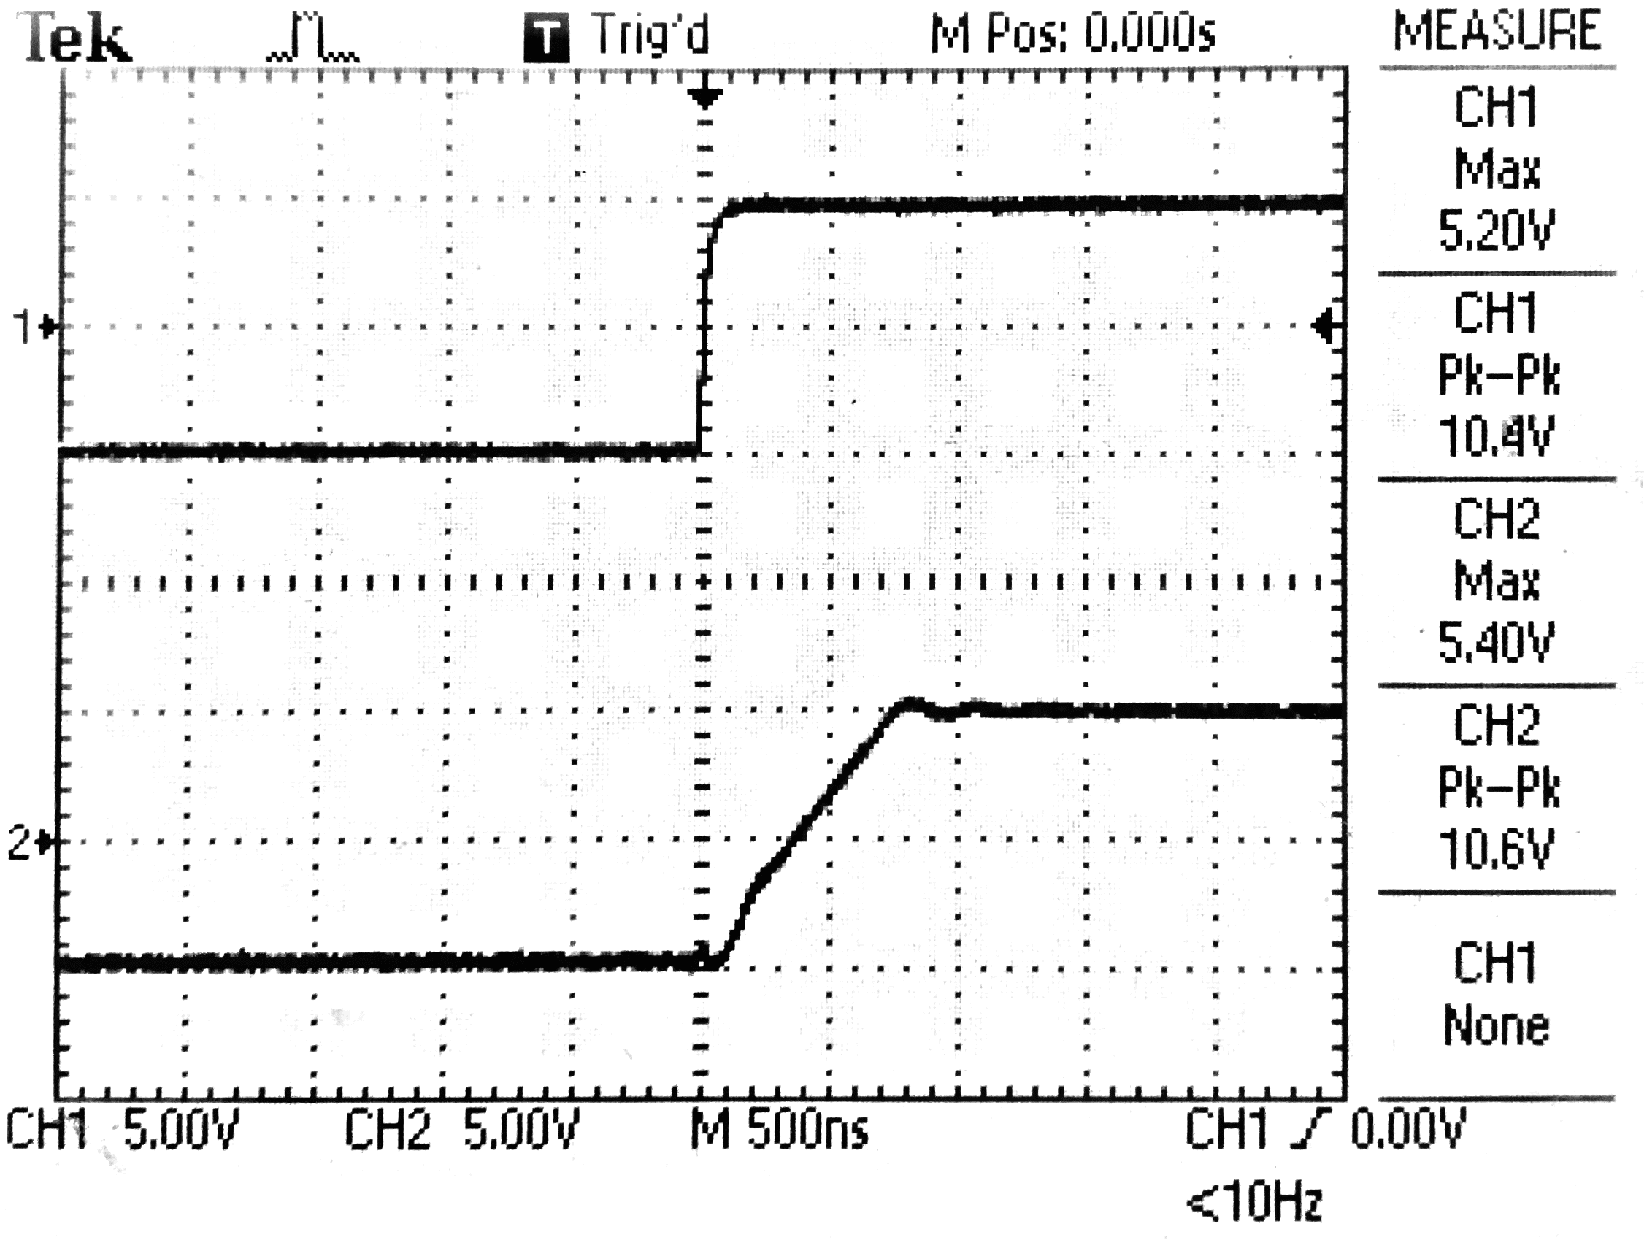
\includegraphics[width=.49\linewidth]{image/rate/slope.pdf}}
            \caption{Measure the slew rate}
            \label{fig:slewRate}
        \end{figure}
        \subsubsection{Disform of sine wave}
            To measure the slew rate, we notice the change for a sinewave is hugh near the point $V(t) = 0$. At a high frequency, the voltage chagne is too quick such that the opamp cannot follow, which cause a disform of sine wave in the output. This can help us to find the slew rate.

            In this part, we use a follower as Figure~\ref{fig:follower}. We use a sine wave as input and find out when the disform happen. We see the peak of the sine wave is start to disform at a frequency of 450kHz and 5V amplitude, as in Figure~\ref{fig:slewRate}a.
        \subsubsection{Sudden voltage change}
            A sudden voltage change can also give us a chance to observed the slew rate. In the lab, we use a follower as in Figure~\ref{fig:follower}. We apply a square wave in the input and find hot how the output delay when the voltage jump from $-V_0$ to $V_0$. THe result obtained is in Figure~\ref{fig:slewRate}b. We see that the voltage change is 10V and the time it takes is 0.8(1)$\mu$s.
\section{Analysis}
    \subsection{Follower}
        We obtained a perfect result. The output is exactly same as the ouput in all frequency and DC. Different than the follower with BJT transistor, the opamp follower does not have a 0.6V voltage drop on the output.

        When we use a load resistor. We see that the output voltage is same as without load resistor. However, when we remove the follower, connect the load resistor directly to the voltage divider, we observed a huge voltage drop on load resistor. This prove that the impedance of our follower is ideal. This is a well functioning follower.
    \subsection{Amplifier}
        We have used two different amplifier. We do achieve a 26dB amplifier. From the data, we see that at higher frequency, the output voltage drop significantly for all different gain, which means the gain is become smaller. This follow the first limit of opamp.

        On the other hand, from Figurer~\ref{fig:amplifierLab}c, we see that the inverting amplifier indeed inverting the input.
    \subsection{Integrator and Differentiator}
        The integrator worked well on different wave form, as in Figure~\ref{fig:integratorWave}. The frequency range it can be used is 100Hz without the T network and is 300Hz with the T network. We also see that the T network slow sheft speed.

        When measure the input and output voltage for square wave, we see that the output voltage drop significantly follow the first limit of opamp.

        The differentiator have a good result for all wave form as in Figure~\ref{fig:differentiatorWave}. We see that for square wave the result is very interesting. The shape we achieve is since the derivative of a square wave with amplitude $A$ is a delta function. The area below the this delta fucntion is proportional to the amplitude of square wave. However, for the opamp, the output voltage cannot go higher than $V-\text{CC}$, which is much less than the height of a delta fucntion. Nevertheless, it have to output the whole delta fucntion, that is to say, the area below the output have to be same as the derivative delta. Thus we see this have square shape in the output.
    \subsection{Slew Rate}
        For the first method, we find $\max\left(\frac{\de V}{\de t}\right) = A \omega$. This give us $450\text{kHz}\times 2 \pi \times 5 V \approx$ 14,000,000 V/s

        For the ohter method, we can jsut calculate the slope as $10\text{V} / 0.8\mu\text{s} \approx$  12,500,000 V/s

\section{Conclusion}
    The result of this lab is good. Follower, inverting and non-inverting amplifier, integrator, and differentiator work as we expect. We can use a large ratio on the T network to improve integrator to slow the shift.



\bibliography{cite}
\bibliographystyle{apsrev4-1}

    % \begin{figure}[h]
    %     \centering
    %     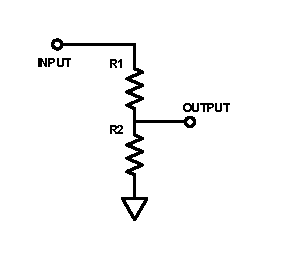
\includegraphics{images/plot2.pdf}
    %     \caption{A voltage divider}
    %     \label{fig:2}
    % \end{figure}

    % \begin{table}[h]
    % \begin{ruledtabular}
    % \begin{tabular}{cccc} 
    % Load[k$\Omega$] &  Output Voltage[V] & $R_\text{th}[\Omega]$ & Theoretical Voltage\\ \hline\hline
    % 50              & 0.680(1)           & 501(1)                & 0.682 \\ \hline
    % 500             & 3.75(1)            & 500(1)                & 3.75 \\ \hline
    % 5000            & 6.80(1)            & 514(1)                & 6.82 \\
    % \end{tabular}
    % \end{ruledtabular}
    % \caption{Load resistor and the output}
    % \label{table:8}
    % \end{table} 

% \begin{center}
%  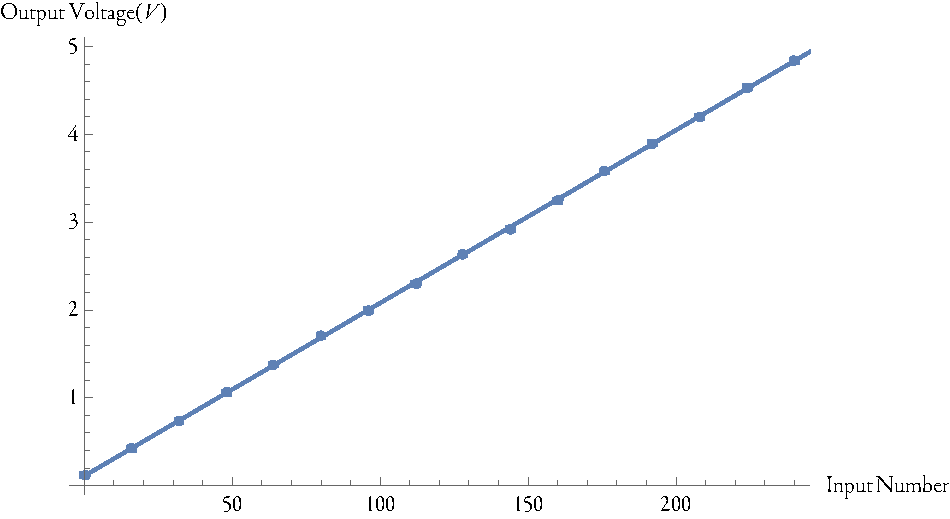
\includegraphics[height=1.8in]{plot.pdf}
% \end{center} 

%\begin{center}
% 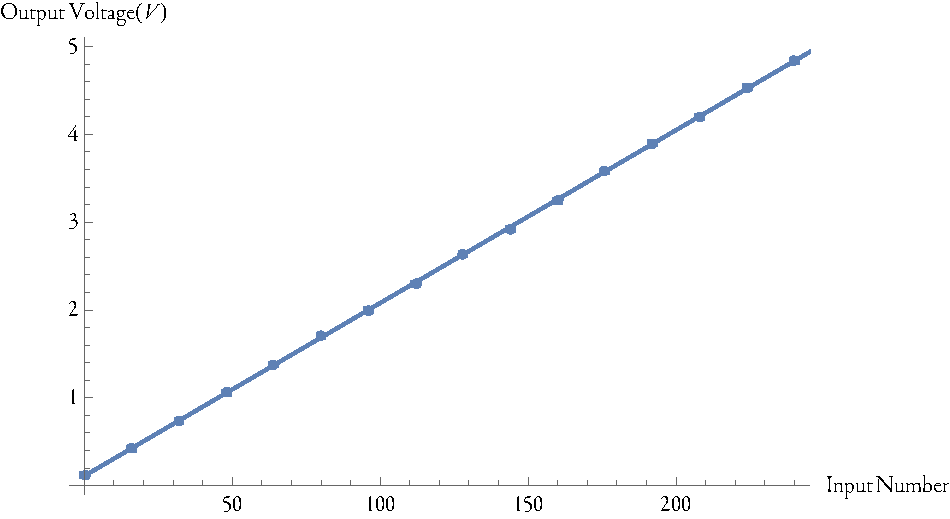
\includegraphics[height=1.3in]{plot.pdf}
%\end{center}

% \blindtext \cite{article-minimal}

% \bibliographystyle{apsrev4-1} % Tell bibtex which bibliography style to use
% \bibliography{xampl} % Tell bibtex which .bib file to use (this one is some example file in TexLive's file tree)

\end{document}